\documentclass[11pt,a4paper]{article}
\usepackage[margin=2.0cm,headsep=0.5cm]{geometry}
\usepackage[T1]{fontenc}
\usepackage[utf8]{inputenc}
\usepackage{amsmath,amssymb,lmodern,microtype,booktabs,longtable,array,xcolor,enumitem,tikz,pgfplots,tcolorbox,fancyhdr,titlesec,graphicx,float,ragged2e,multicol,needspace,pdflscape,textcomp}
\usepackage[colorlinks=true,linkcolor=acc,urlcolor=acc,citecolor=acc]{hyperref}
\usepackage{url}
\pgfplotsset{compat=1.16}
\usetikzlibrary{arrows.meta,positioning,shapes.geometric,calc,fit}
\definecolor{acc}{HTML}{1F4E79}\definecolor{ok}{HTML}{2E7D32}\definecolor{warn}{HTML}{B26A00}\definecolor{bad}{HTML}{B3261E}\definecolor{mid}{HTML}{5A5A5A}
\titleformat{\section}{\Large\bfseries\color{acc}}{\thesection}{0.6em}{}
\titleformat{\subsection}{\large\bfseries\color{acc}}{\thesubsection}{0.5em}{}
\titleformat{\subsubsection}{\normalsize\bfseries\color{acc}}{\thesubsubsection}{0.5em}{}
\setlist{itemsep=2pt,topsep=3pt}
\pagestyle{fancy}\fancyhf{}\fancyfoot[C]{\thepage}\fancyhead[L]{\small C001 quirks: Stage 2, Phase 1}\fancyhead[R]{\small Report, 7 Oct 2026}
\fancypagestyle{lscape}{\fancyhf{}\fancyfoot[C]{\thepage}}
\renewcommand{\arraystretch}{1.12}
\setlength{\tabcolsep}{4pt}
\setlength{\emergencystretch}{3em}
\setlength{\LTcapwidth}{\textwidth}\setlength{\LTpre}{4pt}\setlength{\LTpost}{6pt}
\newtcolorbox{key}[1][]{colback=acc!6,colframe=acc,boxrule=0.6pt,arc=2pt,left=6pt,right=6pt,top=4pt,bottom=4pt,#1}
\newtcolorbox{caution}[1][]{colback=warn!8,colframe=warn,boxrule=0.6pt,arc=2pt,left=6pt,right=6pt,top=4pt,bottom=4pt,#1}
\newtcolorbox{good}[1][]{colback=ok!6,colframe=ok,boxrule=0.6pt,arc=2pt,left=6pt,right=6pt,top=4pt,bottom=4pt,#1}
\newcolumntype{L}[1]{>{\RaggedRight\arraybackslash}p{#1}}
\newcolumntype{C}[1]{>{\centering\arraybackslash}p{#1}}
% ---- macros
\newcommand{\arx}[1]{\href{https://arxiv.org/abs/#1}{arXiv:#1}}
\newcommand{\ax}[1]{\href{https://arxiv.org/abs/#1}{#1}}
\newcommand{\EST}{\textsc{estimate}}
\newcommand{\UNV}{\textsc{unverified}}
\newcommand{\VAPI}{\textsc{verified(api)}}
\DeclareRobustCommand{\file}[1]{\path{#1}}
\newcommand{\mQ}{m_Q}
\newcommand{\NIC}{N_{\mathrm{IC}}}
\newcommand{\GeV}{\,\mathrm{GeV}}
\newcommand{\TeV}{\,\mathrm{TeV}}
\newcommand{\keV}{\,\mathrm{keV}}
\newcommand{\fb}{\,\mathrm{fb}}
\newcommand{\pb}{\,\mathrm{pb}}
\newcommand{\fbinv}{\,\mathrm{fb}^{-1}}
\newcommand{\abinv}{\,\mathrm{ab}^{-1}}
\newcommand{\QQ}{Q\bar Q}
\newcommand{\pTQQ}{p_T(Q\bar Q)}
\newcommand{\ns}{\,\mathrm{ns}}
\newcommand{\um}{\,\mu\mathrm{m}}
\newcommand{\catA}{\textcolor{bad}{\textbf{A}}}
\newcommand{\catB}{\textcolor{warn}{\textbf{B}}}
\newcommand{\catC}{\textcolor{mid}{\textbf{C}}}
\newcommand{\lab}[1]{\textbf{[#1]}}

\begin{document}
\begin{titlepage}
\centering\vspace*{2.2cm}
{\Huge\bfseries\color{acc} Colour-neutral quirks\\[6pt] in the CMS tracker}\\[0.9cm]
{\Large Candidate C001, Stage 2 / Phase 1:\\[3pt] analysis strategy, Phase-2 sample plan,\\[3pt] and two rounds of independent review}\\[1.4cm]
{\large Report on the Phase-1 (Strategy) work}\\[0.5cm]
{\large 7 October 2026}\\[1.6cm]
\begin{minipage}{0.84\textwidth}\small
\begin{key}
\textbf{Status: Phase 1 PASS.} Round-1 review: ITERATE (2 Category-A, 9 Category-B items). Round-2 review by a fresh reviewer: PASS (no Category A; 3 new Category-B items, applied in strategy v3). Nothing has been run on CMS data or CMS simulation yet; this is a design document.
\end{key}
\vspace{4pt}
\textbf{Benchmark:} $E=(1,1)_{-1}$ vector-like Dirac fermion quirk, $\NIC=2$, $\Lambda\equiv\sqrt{\sigma}$ in 0.3--30\,keV, $\mQ\approx 0.2$--$1.25\TeV$, Drell--Yan production.\\[3pt]
\textbf{Experiment:} CMS (Run~3 data and the Phase-2 detector at pile-up 200).\\[3pt]
\textbf{Workspace:} \file{hllhc_search/stage2_C001_quirks/}. Methodology: JFC (phase $\to$ written artifact $\to$ independent review $\to$ fix $\to$ next phase).\\[3pt]
\textbf{Source of every number:} the v3 Phase-1 artifacts (\file{STRATEGY_DRAFT.md}, \file{OPEN_QUESTIONS.md}, \file{SAMPLE_REQUIREMENTS.md}) and the two review files. Labels \EST{} and \UNV{} are kept wherever the sources use them.
\end{minipage}
\vfill
{\small Prepared for the USFQ CMS group; may be shared with colleagues and conveners.}
\end{titlepage}

% ======================================================================
\section*{Executive summary}
\addcontentsline{toc}{section}{Executive summary}
\vspace{-4pt}
{\small
\begin{key}
\textbf{Where we are.} The Phase-1 strategy for a CMS search for colour-neutral, electroweak-charged \emph{quirks} has passed the JFC gate after two independent critical reviews. The first review (ITERATE) found two genuine errors and nine weaknesses; all were fixed, and a fresh second reviewer verified the fixes, recomputed 17 numbers independently, and returned PASS with three further non-blocking items, which were applied (v3). Phase~2 (Exploration) can start once the user makes three blocking decisions (below).
\end{key}

\textbf{The target.} A pair of heavy quirks bound by a keV-scale flux tube crosses the tracker as two slow, heavily ionising, mutually bending, \emph{coplanar} tracks that oscillate about each other. No Standard-Model process produces this pattern. The only LHC limit is FASER's: $\mQ<57$--$179\GeV$ for $\Lambda=0.3$--$30\keV$. No ATLAS or CMS result exists.

\textbf{Key findings.}
\begin{enumerate}[leftmargin=1.4em,itemsep=1pt]
\item \textbf{ATLAS has an active quirk search} (public code trail, Aug--Sep 2026: Geant4 quirk fixes merged into Athena 24.0, an ML pair finder, an internal sensitivity contour). Result \EST{} 2028--29. ``First LHC central-detector quirk search'' is very likely gone.
\item \textbf{The coplanar method works only in a mass-dependent $\Lambda$ window at 3.8\,T}: nominally 0.6--15\,keV at $\mQ\approx500\GeV$; $\approx0.55$--11\,keV at 200\,GeV and $\approx0.8$--19\,keV at 1\,TeV (\EST).
\item \textbf{Heavy pairs are slow and arrive late.} Median delay at the timing-layer radius $\approx16\ns$ (500\,GeV) and $\approx33\ns$ (1\,TeV). \emph{New:} the default CMSSW Phase-2 digitizer drops outer-tracker hits more than 12.5\,ns late, so default simulation silently loses high-mass signal (open item OI-1).
\item \textbf{Cross section} $\sigma(pp\to E\bar E)=6.11\fb$ at 500\,GeV, 14\,TeV (\EST), about $3\times$ the earlier gate estimate.
\item \textbf{Reach depends on the background} (expected 95\% CL, $\Lambda=3\keV$): Run~2 (2017--18) + Run~3: $\approx0.72$--$0.87\TeV$. Phase~2, $3\abinv$: $\approx1.2\TeV$ with zero background, 0.94--0.97\,TeV at the $\mu=50$ background rate, but only $0.57\TeV$ if pile-up 200 multiplies that rate by 16 and the background is known to 20\%. Phase~2 beats Run~2+3 only if the pile-up-200 background is controlled.
\item \textbf{Trigger.} The baseline MET trigger gives $\varepsilon\approx0.1$; a lowered L1 MET threshold gives 0.15--0.25. A muon-system slow-pair seed is \emph{not} ISR-independent and helps mainly at low mass.
\item \textbf{Data access may be cheap:} CMSSW defines RAW-RECO and cluster-level MET skims (\texttt{EXOHighMET}, \texttt{EXOMONOPOLE}) for Run~2 and Run~3. Whether they were produced is \UNV{} (DAS check).
\end{enumerate}

\textbf{Recommendation (provisional, user decision): S3, staged.} Build the common tools (quirk Geant4 port to CMSSW, hit dumper, plane finder, GNN), deliver a CMS Phase-2 sensitivity study, and meanwhile \emph{measure} the random-coplanarity background in Run-3 data; decide at month $\sim$9 whether to launch a full Run-3 search.

\textbf{Decisions needed now (blocking).} \textbf{Q1} scope (S1/S2/S3); \textbf{Q2} check CADI/CDS/McM/DAS for a CMS-internal quirk effort and contact the EXO-LLP conveners; \textbf{Q3} manpower, a SimG4 co-developer, and compute. See Section~\ref{sec:decisions}.
}

\newpage
{\setcounter{tocdepth}{1}\tableofcontents}
\vspace{8pt}

% ======================================================================
\section{Reading guide}\label{sec:reading}
This report is a curated summary. The Markdown files are the authoritative record; when in doubt, they win (and among them, the v3 Phase-1 artifacts win over the research reports). Table~\ref{tab:files} lists the files in the recommended reading order.

\subsection{What to read, in which order}
{\small
\begin{longtable}{@{}L{4.4cm}L{6.3cm}L{1.6cm}L{3.4cm}@{}}
\caption{Files of the Phase-1 work, in recommended reading order. Sizes are on disk on 7 Oct 2026.}\label{tab:files}\\
\toprule
File & What it contains & Size & Read it if\ldots\\\midrule\endfirsthead
\toprule File & What it contains & Size & Read it if\ldots\\\midrule\endhead
\bottomrule\endfoot
1.~\file{phase1_strategy/outputs/STRATEGY_DRAFT.md} (v3) & The strategy itself: physics, scope options, reach, observables, two reconstruction approaches, trigger, backgrounds, systematics, statistics, risks, label registry, and the response to both reviews. \textbf{Start with Sec.~1 (summary), 6 (scope and reach), 10.4 (late-hit open item), 16 (risks), 20 (response to review).} & 91\,kB, 831 lines & always; it is the main deliverable\\
2.~\file{phase1_strategy/outputs/OPEN_QUESTIONS.md} & Q1--Q13 for the user, each with options and a recommendation; Q1--Q3 block Phase~2. & 8.6\,kB & you need to decide something\\
3.~\file{phase2_exploration/outputs/SAMPLE_REQUIREMENTS.md} & Which samples Phase~2 needs, what exists publicly or in CMS, CPU/storage, software work items W1--W12, DAS queries, a 4-week plan. & 24.7\,kB & you will request or produce samples\\
4.~\file{literature/literature_map.md} (+ \file{bibliography.json}, 58 entries) & Literature census: counts, lineage, open problems, code releases, 10 must-read papers, query log. & 14.3\,kB (+38\,kB) & you want the literature context\\
5.~\file{phase1_strategy/review/STRATEGY_CRITICAL_REVIEW.md} & Round-1 review (ITERATE): 32-entry spot-check table, items A1--A2, B1--B9, C1--C8. & 24.0\,kB & you want to see what was wrong in v1\\
6.~\file{phase1_strategy/review/STRATEGY_CRITICAL_REVIEW_R2.md} & Round-2 review (PASS): verification of every round-1 fix, 17 independent recomputations, new B1--B3, C1--C7. & 16.8\,kB & you want to know how the fixes were checked\\
7.~\file{research/theory_signal_model.md} & Background: benchmark choice, cross sections, quirk dynamics, signature map, signal systematics, grid. & 61.8\,kB & reference only (see warning)\\
8.~\file{research/experimental_status_2026.md} & Background: ATLAS code trail, other experiments, reference analyses, Phase-2 trigger and detector facts, backgrounds. & 61.7\,kB & reference only (see warning)\\
9.~\file{research/samples_and_tools.md} & Background: public tools and datasets, CMS-internal resources, proposed environments. & 40.2\,kB & reference only (see warning)\\
10.~\file{LOG.md} & Append-only chronology of the whole stage (agents launched, results, interruption, reviews). & 6.8\,kB & you want the timeline\\
\end{longtable}
}

\begin{caution}
\textbf{The three \file{research/*.md} reports still contain errors that were corrected downstream} and were deliberately not edited: the pair-velocity column of the theory report (Tab.~4.3, $\beta_T$), its edge-point count (Sec.~7), the FASER ISR/MC-statistics attribution in the experimental report (Sec.~4 item~5), its muon-seed efficiency (Sec.~3.6), and the $Z(\nu\nu)$ cross section in the samples report (Sec.~3.0). STRATEGY v3 Sec.~20 lists them. Never take a number from these three files without checking it against STRATEGY v3.
\end{caution}

\subsection{File tree}
{\small
\begin{verbatim}
hllhc_search/                       discovery phase (Gates 1-4, arbiter ranking)
  research/cache/pdf/               cached arXiv PDFs as text (shared by all stages)
  research/tools/                   inspire.py, arxiv_pdf.py
  research/reviews/{theory,experimental,feasibility}/C001.md   Gate-4 reviews
  stage2_C001_quirks/               THIS STAGE
    README.md, LOG.md
    literature/        bibliography.json, literature_map.md
    research/          theory_signal_model.md, experimental_status_2026.md,
                       samples_and_tools.md          (background reports, not edited)
    phase1_strategy/outputs/   STRATEGY_DRAFT.md (v3), OPEN_QUESTIONS.md
    phase1_strategy/review/    STRATEGY_CRITICAL_REVIEW.md (R1),
                               STRATEGY_CRITICAL_REVIEW_R2.md (R2)
    phase2_exploration/outputs/ SAMPLE_REQUIREMENTS.md
    report/            this report (.tex, .pdf)
\end{verbatim}
}

\subsection{The JFC phase layout}
The work follows the JFC methodology (\file{jfc/src/methodology/02-phases.md}). An analysis passes through five phases, each closed by a written artifact and a gate. Table~\ref{tab:jfc} shows where this stage sits.

{\small
\begin{longtable}{@{}L{3.03cm}L{6.48cm}L{3.14cm}L{3.45cm}@{}}
\caption{JFC phases and the status of C001.}\label{tab:jfc}\\
\toprule Phase & Content & Artifact / gate & C001 status\\\midrule\endfirsthead
\bottomrule\endfoot
1 Strategy & signal, backgrounds, observables, $\geq2$ approaches, technique choice, full systematic plan, reference analyses with published numbers, [A]/[L]/[D] labels & \file{STRATEGY.md}; 1 critical reviewer & \textbf{done, PASS} (file named \file{STRATEGY_DRAFT.md})\\
2 Exploration & sample inventory, data quality, closure test, variable survey, baseline yields & \file{EXPLORATION.md}; self-review & prepared: \file{SAMPLE_REQUIREMENTS.md}; not started\\
3 Processing & selection, $\geq2$ approaches compared, CR/VR, background estimate & \file{SELECTION.md}; 1 reviewer & ---\\
4a/4b/4c Statistics & expected (Asimov), 10\% data (human gate), full data & inference notes + analysis note & ---\\
5 Documentation & final analysis note & AN + PDF & ---\\
\end{longtable}
}
The JFC review vocabulary (Category A/B/C, PASS/ITERATE) is explained in Section~\ref{sec:review}.

% ======================================================================
\section{How the work was done}\label{sec:how}
\subsection{Workflow}
The stage ran on 7 October 2026, after the user picked C001 at the discovery-phase checkpoint and confirmed CMS membership (so the strategy targets CMS; public tools are for prototyping only). Figure~\ref{fig:workflow} shows the flow.

\begin{figure}[H]\centering
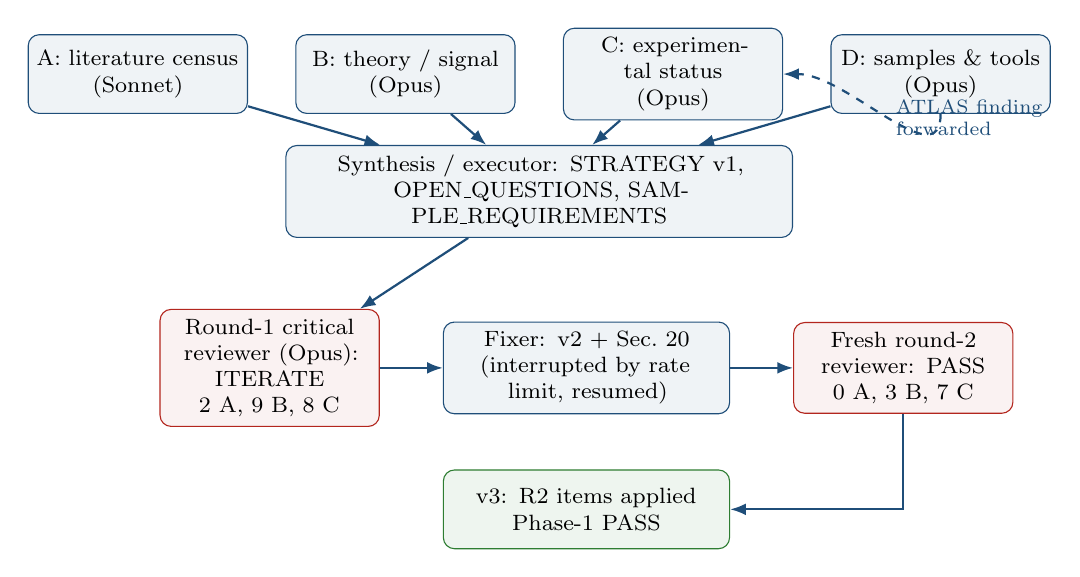
\begin{tikzpicture}[node distance=5mm and 6mm,
  box/.style={draw=acc,fill=acc!7,rounded corners,align=center,minimum height=1.0cm,font=\footnotesize,text width=2.55cm},
  rev/.style={draw=bad,fill=bad!6,rounded corners,align=center,minimum height=1.0cm,font=\footnotesize,text width=2.55cm},
  arr/.style={-{Latex[length=2mm]},thick,acc}]
\node[box](a){A: literature census\\(Sonnet)};
\node[box,right=of a](b){B: theory / signal\\(Opus)};
\node[box,right=of b](c){C: experimental status\\(Opus)};
\node[box,right=of c](d){D: samples \& tools\\(Opus)};
\node[box,below=9mm of $(b)!0.5!(c)$,text width=6.2cm](s){Synthesis / executor: STRATEGY v1,\\ OPEN\_QUESTIONS, SAMPLE\_REQUIREMENTS};
\node[rev,below left=9mm and -1.2cm of s](r1){Round-1 critical reviewer (Opus): ITERATE\\2 A, 9 B, 8 C};
\node[box,right=8mm of r1,text width=3.4cm](f){Fixer: v2 + Sec.~20\\(interrupted by rate limit, resumed)};
\node[rev,right=8mm of f](r2){Fresh round-2 reviewer: PASS\\0 A, 3 B, 7 C};
\node[box,below=7mm of f,text width=3.4cm,fill=ok!8,draw=ok](v3){v3: R2 items applied\\Phase-1 PASS};
\draw[arr](a)--(s);\draw[arr](b)--(s);\draw[arr](c)--(s);\draw[arr](d)--(s);
\draw[arr](s)--(r1);\draw[arr](r1)--(f);\draw[arr](f)--(r2);\draw[arr](r2)|-(v3);
\draw[arr,dashed](d.south) to[out=-90,in=0] node[right,font=\scriptsize,align=left]{ATLAS finding\\forwarded} (c.east);
\end{tikzpicture}
\caption{Workflow of the stage. Agents B, C and D exchanged two findings during the run (the ATLAS code trail went from D to C; the late-hit timing threat went from B to C).}\label{fig:workflow}
\end{figure}

\begin{enumerate}
\item \textbf{Four parallel research agents} wrote the background reports: A, literature census (\file{literature/}); B, theory and signal model; C, experimental status, Phase-2 trigger and detector plan, reference analyses; D, samples and tools.
\item \textbf{A synthesis agent (executor)} wrote STRATEGY v1, OPEN\_QUESTIONS and SAMPLE\_REQUIREMENTS. It re-read every number in the report it came from, re-checked a sample of load-bearing numbers against the cached primary PDFs, logged ten conflicts between the reports (STRATEGY Sec.~2.4, C1--C10), and made three small read-only checks of the CMSSW source (C7--C9).
\item \textbf{An independent critical reviewer} (JFC \file{agents/critical_reviewer.md}) who had not written the artifacts checked them against the research files, the cached PDFs, HEPData, and the live CMSSW, Athena and GitHub repositories. Verdict: ITERATE.
\item \textbf{A fix pass} addressed every A and B item and wrote STRATEGY Sec.~20 ``Response to review'' (v2).
\item \textbf{A fresh reviewer} (who had done neither the artifacts nor round~1) verified each fix and recomputed numbers independently. Verdict: PASS, with three new B items, which were applied (v3, STRATEGY Sec.~20.2).
\end{enumerate}

\textbf{Models.} Agent A (literature census) ran on Sonnet. Agents B, C and D, the synthesis executor (which also did both fix passes, as the same resumed agent), the round-1 reviewer, the fresh round-2 reviewer and the report writer all ran on Opus. The orchestrator (Opus) delegated the work and spot-checked the ATLAS evidence itself.

\subsection{Tools and sources}
\begin{itemize}
\item \textbf{INSPIRE} REST API (project tool \file{inspire.py}: searches, citer lists \texttt{refersto:recid}); about 590 candidate records were screened for the census.
\item \textbf{arXiv PDFs} downloaded and converted to text (\file{arxiv_pdf.py}, cache \file{research/cache/pdf/}); reviewers quote these at line level (e.g.\ ``2410.09164 l.986--987'').
\item \textbf{HEPData} (FASER record \texttt{ins3184325}, table t2, exclusion contour).
\item \textbf{GitHub and CERN GitLab APIs}: \texttt{burzynski-lab/quirk-tracking} and \texttt{quirkviz}, Athena merge requests and files, public ML code repositories.
\item \textbf{CMSSW source} (cms-sw/cmssw master, read via the API): skim definitions, Phase-2 digitizer, event content, geometry list.
\item Zenodo, HuggingFace (ColliderML), CERN Open Data and \texttt{pixi search} for datasets and packages; web search for talks and approval status.
\item Not reachable: \textbf{CDS} (blocked by a bot challenge), and therefore any CMS-internal source (CADI, CDS notes, twikis). No CMS RAG corpus was available.
\end{itemize}

\subsection{Evidence rules}
Every number in the artifacts must carry one of:
\begin{itemize}
\item a citation \texttt{[ID, location]}, e.g.\ \texttt{[1708.02243 Sec.~IV]} or \texttt{[HEPData ins3184325 t2]};
\item \EST: a calculation by an agent of this project, with its inputs stated or referenced;
\item \UNV: recalled or read from a secondary source, not checked against the primary source;
\item \VAPI: read from a live public repository or API on 2026-10-07.
\end{itemize}
Statements that the analysis depends on carry JFC labels: \lab{A} \emph{assumption} (a premise taken as true; must be validated or carried as a systematic), \lab{L} \emph{limitation} (a known shortfall with its impact; goes to the analysis note), \lab{D} \emph{decision} (a binding choice with its reason; a silent change of a [D] later is Category~A). The registry is in Appendix~\ref{app:labels}.

\subsection{Interruption}
At 17:10 the fix pass after review round~1 was \textbf{interrupted by the session rate limit} (HTTP 429; reset at 21:00 America/Guayaquil). At that point STRATEGY\_DRAFT was partly revised (status line ``v2'', no Sec.~20), and SAMPLE\_REQUIREMENTS and OPEN\_QUESTIONS were not yet revised. The log recorded the state and the resume instruction; after the reset the fix pass was re-run for all A/B items, Sec.~20 was written, and the fresh round-2 reviewer was launched. 
% ======================================================================
\section{Physics: quirks and the benchmark}\label{sec:physics}
\subsection{What a quirk is}
Take a new confining gauge group SU($\NIC$) (``infracolour'', IC) whose only charged matter is heavy: fermions or scalars $Q$ with mass $\mQ\gg\Lambda$, where $\Lambda$ is the IC confinement scale. Because there are no light IC-charged states, the flux tube between a produced $Q\bar Q$ pair cannot break: the pair stays bound by a string of tension $\sigma$ over macroscopic distances \cite{KL}. If $Q$ also carries Standard-Model electroweak charge, it is produced by Drell--Yan and leaves tracks.

\textbf{Conventions [D1].} $\Lambda\equiv\sqrt{\sigma}$, i.e.\ $\sigma=\Lambda^2$ \cite{Knapen}. The cosmology paper \cite{cool} uses $\Lambda=T_c\approx0.6\sqrt\sigma$; its bounds are converted by $\times1/0.6$. The oscillation length is taken from the exact energy-conservation result for a straight string,
\begin{equation}
\ell_{\max}=\frac{2(\gamma^*-1)\,\mQ}{\sigma}=3.95\,\mathrm{cm}\times(\gamma^*-1)\left(\frac{\mQ}{100\GeV}\right)\left(\frac{\mathrm{keV}}{\Lambda}\right)^{2},
\end{equation}
where $\gamma^*$ is the Lorentz factor of each quirk in the pair rest frame at production. The shorthands used in the literature differ from this by factors 2--4 and are not used. Results are quoted per $(\mQ,\Lambda)$ for $\NIC=2$, with cross-section limits per unit $\NIC$ so that $\NIC=3,5$ follow by rescaling.

\subsection{Why the keV window}
\begin{itemize}
\item \textbf{Generic hidden confinement.} $\Lambda$ is log-flat in the UV coupling. The whole target window 0.3--30\,keV corresponds to $\alpha_{\rm IC}(\mQ)\approx0.040$--0.052, a $\sim$25\% coupling range (\EST) \cite{KL}.
\item \textbf{Neutral naturalness} motivates quirks, but with GeV-scale $\Lambda$. The mesoscopic (keV) window is therefore \emph{signature-driven, not naturalness-driven} \lab{A1}, and the strategy says so plainly.
\item \textbf{Cosmology.} Nothing excludes the target region; a discovery would imply a low reheating temperature, $T_{\rm RH}\lesssim\mathcal{O}(100\GeV)$ \cite{cool}. This adds motivation; it is not a constraint.
\item \textbf{Experimental gap.} Only FASER, D0 and an old HSCP/monojet recast constrain the region (Section~\ref{sec:limits}); no ATLAS/CMS publication exists.
\item \textbf{Distinctiveness.} Two mutually bending, coplanar, slow, $\sim$2--10$\times$ MIP tracks. No HSCP, R-hadron, monopole, multi-charge or disappearing-track signature looks like this. Once observed, a trajectory fit measures $\mQ$ and $\Lambda$ \cite{Knapen}.
\end{itemize}

\subsection{Regimes in $\Lambda$}
The topology is set by $\ell_{\max}$ compared with the tracker size and with the hit resolution. Table~\ref{tab:regimes} gives the regime map for CMS at 3.8\,T (STRATEGY Sec.~4.3, \EST{} unless cited). The edges depend on $\mQ$ (next subsection).

{\small
\begin{longtable}{@{}L{3.34cm}L{5.06cm}L{3.44cm}L{4.25cm}@{}}
\caption{Regime map in $\Lambda$ for the CMS tracker at 3.8\,T.}\label{tab:regimes}\\
\toprule $\Lambda$ & Topology & Primary tool & Notes\\\midrule\endfirsthead
\bottomrule\endfoot
$\lesssim0.2\keV$ & $\ell_{\max}\gtrsim1$\,m, nearly helical & HSCP searches & out of scope \lab{D4}\\
0.3\,keV to $\Lambda_{\rm low}(\mQ)$ & 1--5 string crossings; plane thicker than 100\,$\mu$m (0.1--5\,mm) & trajectory $\chi^2$ fit / GNN & coplanar finder fails; FASER weak here (57--72\,GeV)\\
\textbf{$\Lambda_{\rm low}(\mQ)$ to $\Lambda_{\rm high}^{\rm OT}(\mQ)$} (nominal ``0.6--15\,keV'' at 500\,GeV) & $10^1$--$10^3$ crossings, plane thickness $\leq100\um$, two hits per layer resolved in IT and OT & \textbf{coplanar plane finder} + dE/dx + timing & core window\\
$\Lambda_{\rm high}^{\rm OT}$ to $\Lambda_{\rm high}^{\rm IT}$ & pair merged in OT $r\phi$, resolved in IT & IT-only plane + dE/dx & degrading\\
$\gtrsim\Lambda_{\rm high}^{\rm IT}$ ($\approx$20--40\,keV) & one straight, $\geq2\times$ MIP, ``infinite-$p_T$'' track & straight-pair / highly-ionising selection & FASER covers up to 100\,keV\\
\end{longtable}
}

\subsection{Window edges versus $\mQ$}\label{sec:edges}
Both edges were derived in v2 after review item B2 (STRATEGY Sec.~4.4; \EST).

\textbf{Lower edge (plane thickness).} The two quirks oscillate in a plane whose thickness is \cite{LiLi}
\begin{equation}
d\approx1.16\um\left(\frac{\mQ}{100\GeV}\right)\left(\frac{\mathrm{keV}}{\Lambda}\right)^{4}\left(\frac{B_{xy}}{\mathrm{T}}\right).
\end{equation}
Requiring $d$ below Knapen's $\Delta s=100\um$ cut \cite{Knapen} with $B_{xy}=3.8$\,T gives
\begin{equation}
\Lambda_{\rm low}\approx0.458\keV\,(\mQ/100\GeV)^{1/4}=0.54\,/\,0.69\,/\,0.81\keV\quad(\mQ=200/500/1000\GeV).
\end{equation}
The thickness formula is accurate only to about $\times10$ \cite{traj}, i.e.\ $\times10^{\pm1/4}\approx\times1.8$ in $\Lambda$: the bands are 0.31--0.97, 0.39--1.22 and 0.46--1.45\,keV. Using the maximum in-plane field makes $\Lambda_{\rm low}$ conservative (high). At ATLAS (2\,T) the edge at 500\,GeV is 0.58\,keV instead of 0.69\,keV, a small CMS disadvantage.

\textbf{Upper edge (hit merging).} The quirks merge into one hit when their separation falls below the two-hit resolution $s_{\rm res}$:
\begin{equation}
\Lambda_{\rm high}=\left[\frac{3.95\,\mathrm{cm}\,(\gamma^*-1)(\mQ/100\GeV)}{s_{\rm res}}\right]^{1/2}\keV ,
\end{equation}
with median $\gamma^*=1.30/1.25/1.19$. For the outer tracker (OT) $r\phi$, $s_{\rm res}\approx200\um$ gives $\Lambda_{\rm high}^{\rm OT}\approx11/16/19\keV$; for the inner tracker (IT), $s_{\rm res}\approx50\um$ gives $\Lambda_{\rm high}^{\rm IT}\approx22/31/39\keV$ (200/500/1000\,GeV). Since $\ell_{\max}$ is the \emph{maximum} separation, these are upper estimates. Hence ``0.6--15\,keV'' is the nominal window at 500\,GeV; it is $\approx$0.55--11\,keV at 200\,GeV and $\approx$0.8--19\,keV at 1\,TeV. The fast propagator (work item W3) replaces these estimates with efficiency curves in Phase~2.

\begin{figure}[H]\centering
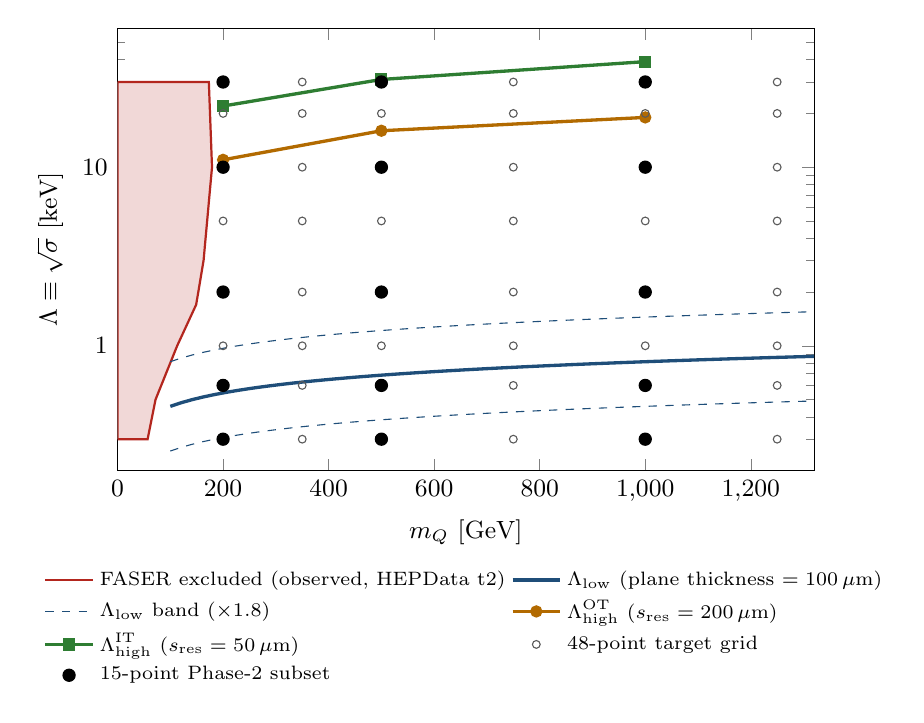
\begin{tikzpicture}
\begin{axis}[width=0.86\textwidth,height=7.2cm,xmin=0,xmax=1320,ymode=log,ymin=0.2,ymax=60,
  xlabel={$\mQ$ [GeV]},ylabel={$\Lambda\equiv\sqrt{\sigma}$ [keV]},
  legend style={font=\scriptsize,at={(0.5,-0.2)},anchor=north,draw=none},legend columns=2,legend cell align=left,
  tick label style={font=\small},label style={font=\small},
  log ticks with fixed point]
\addplot[fill=bad!18,draw=bad,thick] coordinates {(0,0.3)(57,0.3)(72,0.5)(113,1)(149,1.7)(163,3)(179,10)(173,30)(0,30)} -- cycle;
\addlegendentry{FASER excluded (observed, HEPData t2)}
\addplot[acc,very thick,domain=100:1320,samples=60]{0.458*(x/100)^0.25};
\addlegendentry{$\Lambda_{\rm low}$ (plane thickness $=100\,\mu$m)}
\addplot[acc,dashed,domain=100:1320,samples=60,forget plot]{1.778*0.458*(x/100)^0.25};
\addplot[acc,dashed,domain=100:1320,samples=60]{0.458*(x/100)^0.25/1.778};
\addlegendentry{$\Lambda_{\rm low}$ band ($\times1.8$)}
\addplot[warn,very thick,mark=*,mark size=1.6pt] coordinates {(200,11)(500,16)(1000,19)};
\addlegendentry{$\Lambda_{\rm high}^{\rm OT}$ ($s_{\rm res}=200\,\mu$m)}
\addplot[ok,very thick,mark=square*,mark size=1.6pt] coordinates {(200,22)(500,31)(1000,39)};
\addlegendentry{$\Lambda_{\rm high}^{\rm IT}$ ($s_{\rm res}=50\,\mu$m)}
\addplot[only marks,mark=o,mark size=1.4pt,mid] coordinates {
(200,0.3)(200,0.6)(200,1)(200,2)(200,5)(200,10)(200,20)(200,30)
(350,0.3)(350,0.6)(350,1)(350,2)(350,5)(350,10)(350,20)(350,30)
(500,0.3)(500,0.6)(500,1)(500,2)(500,5)(500,10)(500,20)(500,30)
(750,0.3)(750,0.6)(750,1)(750,2)(750,5)(750,10)(750,20)(750,30)
(1000,0.3)(1000,0.6)(1000,1)(1000,2)(1000,5)(1000,10)(1000,20)(1000,30)
(1250,0.3)(1250,0.6)(1250,1)(1250,2)(1250,5)(1250,10)(1250,20)(1250,30)};
\addlegendentry{48-point target grid}
\addplot[only marks,mark=*,mark size=2.2pt,black] coordinates {
(200,0.3)(200,0.6)(200,2)(200,10)(200,30)(500,0.3)(500,0.6)(500,2)(500,10)(500,30)(1000,0.3)(1000,0.6)(1000,2)(1000,10)(1000,30)};
\addlegendentry{15-point Phase-2 subset}
\end{axis}
\end{tikzpicture}
\caption{Regime map at 3.8\,T (\EST). Between the blue line and the orange line the coplanar plane finder works; below the blue band a trajectory fit or GNN is needed; above the green line the pair is one straight, highly ionising track. Edge values from STRATEGY Sec.~4.4; FASER contour from HEPData \texttt{ins3184325} t2; grid from STRATEGY Sec.~7.}\label{fig:regime}
\end{figure}

\subsection{Benchmark and cross sections}
\textbf{Primary benchmark [D3]:} $E=(1,1)_{-1}$ vector-like Dirac fermion, $\NIC=2$, produced by Drell--Yan via $\gamma^*/Z$. It is the common benchmark of FASER, FASER2 projections, Knapen et al., Li et al., Evans--Luty and Farina--Low, so a CMS result overlays on all of them without reinterpretation. It has no charged--neutral splitting and the pair is net neutral (clean coplanarity). Alternates: the scalar $\tilde E$ (spin and kinematics; $\sigma$ smaller by $\times$1/11--1/18; 9 points) and the doublet $L$ (topology only: $Q^\pm\to Q^0\pi^\pm$ with $c\tau\approx7$\,mm, \EST/\UNV; 2 points).

{\small
\begin{longtable}{@{}rrrrr@{}}
\caption{$\sigma(pp\to E\bar E)$ for $\NIC=2$, in fb (\EST: LO CT18NLO $\times$ SUSY-WG K-factor; theory report Sec.~2.3, adopted as the absolute normalisation [D2]). NNLL scale uncertainty $\leq1\%$.}\label{tab:xsec}\\
\toprule $\mQ$ [GeV] & 13\,TeV & 13.6\,TeV & 14\,TeV & PDF4LHC21 unc.\\\midrule\endfirsthead
\bottomrule\endfoot
200 & 193 & 210 & 220 & $\pm3.7\%$\\
500 & 5.16 & 5.70 & 6.11 & $\pm6.6\%$\\
800 & 0.525 & 0.601 & 0.660 & $\pm11.9\%$\\
1000 & 0.148 & 0.176 & 0.197 & $\pm18.5\%$\\
1200 & 0.0469 & 0.0576 & 0.0656 & $\pm25\%$ (extrapolated)\\
\end{longtable}
}
The 500\,GeV value is about $3\times$ the Gate-4 estimate (1.5--2\,fb), which had assumed a fermion/scalar ratio of 4; the computed ratio is 11--18. The trigger needs initial-state radiation (ISR): only $\approx0.10$ of Drell--Yan pairs recoil against a jet with $p_T>200\GeV$ \cite{LiLi,Knapen}.

\subsection{What the pair does in the tracker}
\begin{itemize}
\item \textbf{Dynamics.} Straight-string equations of motion with Lorentz force and ionisation; external forces are $\lesssim$1--4\% of $\Lambda^2$ for $\Lambda\geq0.3\keV$. Glueball emission is negligible in the tracker for $\Lambda\leq30\keV$ ($<0.1\GeV$ of $\sim$100\,GeV internal energy, \EST).
\item \textbf{Ionisation.} Per-hit dE/dx $\approx$2--10$\times$ MIP, tail $\gtrsim50\times$ MIP (\EST); ATLAS-pixel simulation reaches $\sim$60$\times$ MIP \cite{Knapen}. At Phase~2 only the IT measures charge (4-bit ToT); the OT is binary.
\item \textbf{More than two hits per layer} in 10--20\% of events \cite{traj}. Essentially no pairs stop in the tracker; 1--5\% stop in the calorimeters \cite{EvansLuty}.
\item \textbf{Slow pair.} The two quirks move together at the \emph{pair} velocity. Median transverse velocities $v_T=0.38/0.19/0.10$ for $\mQ=200/500/1000\GeV$ at $\pTQQ=250\GeV$, and $0.55/0.34/0.20$ at 500\,GeV (\EST; derived from the theory report's arrival-time column after review item B1).
\end{itemize}
Table~\ref{tab:toa} gives the delay with respect to a $\beta=1$ particle, $t_{\rm oa}=(r/c)(1/v_T-1)$, layer by layer. This is exactly the quantity the CMSSW Phase-2 digitizer cuts on (Section~\ref{sec:oi1}).

{\small
\begin{longtable}{@{}L{2.66cm}C{1.70cm}C{2.87cm}C{3.09cm}C{1.38cm}L{3.83cm}@{}}
\caption{Hit delay $t_{\rm oa}$ in ns for the median pair at $\eta=0$ (\EST; STRATEGY Sec.~4.2). Bold: outside the default $\pm12.5$\,ns OT window. Radii from the Tracker TDR.}\label{tab:toa}\\
\toprule $\mQ$, $\pTQQ$ & IT L4 (15.7\,cm) & PS L1/L2/L3 (24.8/37.2/\allowbreak 52.3\,cm) & 2S L1/L2/L3 (68.7/86.0/110.8\,cm) & BTL {\footnotesize(114.8\,cm)} & OT layers lost with default window\\\midrule\endfirsthead
\bottomrule\endfoot
200, 250\,GeV & 0.8 & 1.3 / 2.0 / 2.8 & 3.7 / 4.6 / 6.0 & 6.2 & none\\
500, 250\,GeV & 2.2 & 3.5 / 5.2 / 7.3 & 9.6 / \textbf{12.0} / \textbf{15.4} & 16.0 & 2S L3 lost; 2S L2 marginal\\
500, 500\,GeV & 1.0 & 1.6 / 2.5 / 3.4 & 4.5 / 5.7 / 7.3 & 7.6 & none\\
1000, 250\,GeV & 4.5 & 7.1 / 10.6 / \textbf{15.0} & \textbf{19.7 / 24.6 / 31.7} & 32.9 & PS L3 and all 2S lost (IT kept)\\
1000, 500\,GeV & 2.1 & 3.3 / 4.9 / 7.0 & 9.1 / 11.4 / \textbf{14.7} & 15.3 & 2S L3 lost\\
\end{longtable}
}
Individual quirks oscillate about the pair centre of mass, so per-hit times scatter around these values; pairs at $|\eta|>0$ have longer paths.

% ======================================================================
\section{Literature, lineage and current limits}\label{sec:lit}
\subsection{The census}
The literature agent screened about 590 INSPIRE records (title, abstract, author and citation queries; the full query list is in the appendix of \file{literature_map.md}) and the PDF text of 40+ papers. \file{bibliography.json} holds 58 entries: about 33 quirk-core papers (theory/model 11, phenomenology projections 14, recasts 2, experimental searches 2, reconstruction tools 3, cosmology/DM 5) and 25 peripheral ones. Ten collider-signature papers deal with the macroscopic/mesoscopic coplanar or forward-timing regime. \textbf{No quirk paper simulates HL-LHC pile-up}: \cite{Knapen} uses $\langle\mu\rangle=50$; \cite{Sha,Condren} explicitly defer pile-up. A limitation: backward references of the newest papers were not run through INSPIRE.

\subsection{Lineage}
{\small
\begin{longtable}{@{}L{1.65cm}L{15.02cm}@{}}
\caption{Chronology of the quirk literature (from \file{literature_map.md} Sec.~2).}\label{tab:lineage}\\
\toprule Year & Papers\\\midrule\endfirsthead
\bottomrule\endfoot
2007--08 & Jacoby--Nussinov \ax{0712.2681} (relic abundance); \textbf{Kang--Luty \ax{0805.4642}}, the founding paper (macroscopic strings, regimes by $\Lambda$); Burdman--Chacko \ax{0805.4667} (folded-SUSY squirkonium); Cai--Cheng--Terning \ax{0812.0843} (quirky little Higgs)\\
2009--11 & quirky dark matter \ax{0909.2034}; \textbf{D0 \ax{1008.3547}} (only pre-LHC search); Harnik--Kribs--Martin \ax{1106.2569}; Fok--Kribs \ax{1106.3101}\\
2015--16 & diphoton-era papers \ax{1512.05753}, \ax{1512.05775}; Chacko--Curtin \ax{1512.05782} (quirky neutral naturalness)\\
2017 & \textbf{Farina--Low \ax{1703.00912}} (HSCP/monojet recast); \textbf{Knapen--Lou--Papucci--Setford \ax{1708.02243}} (coplanar hits in the tracker): together the basis of all later central-detector work\\
2018--20 & Evans--Luty \ax{1811.08903} (stopped quirks); Li--Li et al.\ \ax{1911.02223} (ionisation energy loss in the coplanar search); \ax{2002.07503} (analytic trajectory)\\
2021--24 & Li--Pei \ax{2108.06748} (FASER/FASER2); Li--Liao \ax{2311.15486} (far detectors); Feng--Li et al.\ \ax{2404.13814} (timing at FASER); \textbf{Sha et al.\ \ax{2410.00269}} (GNN reconstruction); FPF@FCC \ax{2409.02163}\\
2025 & Condren--Whiteson \ax{2509.08878} (model-agnostic non-helical tracks); Forsyth--Low \ax{2504.02940}; Curtin--Dreyer \ax{2506.11192}; Asadi--Kribs--Luty \ax{2512.20696} (cosmology: $T_{\rm RH}\lesssim100\GeV$)\\
2026 & Cid Vidal--Fern\'andez G\'omez \ax{2601.09023} (LHCb VELO); \textbf{FASER \ax{2607.26195}} (first LHC quirk search, zero events)\\
\end{longtable}
}
Two author lines dominate: the propagation/far-detector line of Jinmian Li and collaborators, and the tracker-reconstruction line Knapen/Papucci/Setford $\to$ Whiteson group.

\subsection{Must-read papers}
\begin{enumerate}[itemsep=0pt]
\item \arx{1708.02243} Knapen et al.: the coplanar-hit tracker search that is the target; trigger and background arguments at $\mu=50$.
\item \arx{2410.00269} Sha et al.: GNN reconstruction of quirk tracks; pile-up explicitly left open.
\item \arx{2607.26195} FASER: the first and only LHC quirk search; the exclusion to beat.
\item \arx{0805.4642} Kang--Luty: the physics foundation.
\item \arx{1703.00912} Farina--Low: what HSCP/monojet searches exclude; the keV gap.
\item \arx{1911.02223} Li--Li et al.: ionisation-loss improvement; most complete tracker-level simulation of ATLAS/CMS-type setups.
\item \arx{2002.07503} Li--Li et al.: analytic quirk trajectory and plane thickness.
\item \arx{2509.08878} Condren--Whiteson: model-agnostic non-helical tracking and its listed limitations.
\item \arx{2601.09023} LHCb VELO: planar-pattern analysis in a software trigger.
\item \arx{1811.08903} Evans--Luty: stopped quirks and the out-of-time channel.
\end{enumerate}

\subsection{Open problems stated in the literature}
The census extracted the explicit ``future work'' statements and checked their follow-up through citer lists. The relevant ones for this project:
\begin{itemize}
\item \cite{Knapen}: a dedicated trigger and an extension are ``left for future work''. An HL-LHC (pile-up 200) version or an L1/HLT track-trigger version was \emph{not found}.
\item \cite{Sha}: ``Effects from pile-up remain to be studied rigorously in future work''. Not found among its 8 citers. \cite{Condren} addresses model-agnostic tracking at $\mu=1$ only and lists hit noise, misalignment, hard radiation and segment piecing as future work (not found).
\item \cite{FarinaLow}: limits for more quantum numbers (done in the FASER papers); triggering on anomalous tracks; a CMS 0\,T data search (not found).
\item \cite{EvansLuty}: a dedicated out-of-time search to separate quirks from dark matter in monojet (not found).
\item \cite{FASER}: notes that no dedicated LHC search existed before; covers only charge $\pm1$ colourless pairs. ATLAS/CMS follow-up not found in the literature (but see Section~\ref{sec:comp}).
\end{itemize}

\subsection{Code and data releases}
\begin{caution}
\textbf{Inconsistency between sources.} The literature map (written first) concludes that ``no public quirk-propagation or quirk-generation code was found'' and that no ATLAS/CMS quirk activity exists. Both statements were overtaken the same day by the samples and experimental agents, who found the public Athena Geant4 quirk package and the ATLAS code trail. The literature map was not updated; use the list below. (The literature map also reports that the HEPData page returned HTTP 403, whereas the theory agent and the round-1 reviewer did read the FASER HEPData tables.)
\end{caution}
\begin{itemize}
\item \textbf{Athena \file{Simulation/G4Extensions/Quirks}} (Apache-2.0, \VAPI): the only public, collaboration-validated Geant4 quirk transport (\texttt{QuirkTransportation}, \texttt{InfracolorForce}, \texttt{HyperbolaStepper}, a stacking action alternating $Q$/$\bar Q$, a standalone Geant4 test application). FASER adapted it. It must be ported to CMSSW \texttt{SimG4Core} (Section~\ref{sec:samples}). A Geant4-header file inside it must be licence-checked before redistribution.
\item \textbf{Zenodo 17941765}: the \cite{Sha} hit dataset (CC-BY-4.0, 16.4\,GB, 25 $(m,\Lambda)$ points, toy 8/25-layer detector, no pile-up).
\item GNN code \texttt{shaqiyu/QuirkTracking-ML} and \texttt{LeviCondren/Tracking\_pipeline}: public but \emph{without licence} (author permission needed). \texttt{hepattn} (GPL-3.0) and \texttt{acorn} are usable alternatives.
\item FASER HEPData record \texttt{ins3184325} (exclusion contours).
\item Not public: the Knapen--Papucci trajectory/plane-finder code (shared privately), the Li et al.\ EOM solvers and UFOs, the LHCb VELO hit generator.
\end{itemize}

\subsection{Current limits}\label{sec:limits}
{\small
\begin{longtable}{@{}L{4.10cm}L{8.40cm}L{3.89cm}@{}}
\caption{Existing constraints on colour-neutral quirks ($E$-like, $\NIC=2$ unless stated).}\label{tab:limits}\\
\toprule Source & Result & Comment\\\midrule\endfirsthead
\bottomrule\endfoot
FASER, 186\,fb$^{-1}$ \cite{FASER} & observed exclusion 57 / 72 / 113 / 149 / 163 / 179 / 173\,GeV at $\Lambda$ = 0.3 / 0.5 / 1 / 1.7 / 3 / 10 / 30\,keV [HEPData \texttt{ins3184325} t2; checked by the round-1 reviewer: 57.32 / 72.5 / 113 / 149.1 / 162.58 / 179 / 173] & zero events; the only LHC quirk search\\
D0 \cite{D0} & 107\,GeV ($N=2$) for 10\,keV--1\,MeV & unresolved regime\\
Farina--Low recast \cite{FarinaLow} (12.9\,fb$^{-1}$, 2016) & (1,1)$_{-1}$ fermion, $N=2$: 150\,GeV at 100\,eV, \textbf{no bound at 1\,keV} & latest HSCP/monojet recast; no full Run-2/3 recast exists\\
CMS HSCP dE/dx \cite{HSCP} (101\,fb$^{-1}$) & Drell--Yan $\tau'$ with $Q=1e$ (same quantum numbers as $E$) excluded below 1.02\,TeV (ionisation method) and 1.14\,TeV (mass method); $Q=2e$: 1.32 / 1.41\,TeV & the $\Lambda\to0$ anchor; valid only for $\Lambda\lesssim0.1\keV$, and for $\NIC=1$ ($\NIC=2$ roughly $+0.1\TeV$, \EST)\\
\multicolumn{3}{@{}l}{\emph{Projections (comparison targets, not limits)}}\\
Knapen et al.\ \cite{Knapen} & EW quirks up to 650\,GeV (5 events, 300\,fb$^{-1}$, $\mu=50$) & toy ATLAS-like detector\\
Sha et al.\ \cite{Sha} & $N>3$ events for $\mQ\lesssim700\GeV$, $\Lambda\lesssim5\keV$, 300\,fb$^{-1}$, no pile-up & toy detector\\
FASER2 \cite{Feng} & 1.0\,TeV discovery for $E$ at 3\,ab$^{-1}$ & not approved\\
\end{longtable}
}

% ======================================================================
\section{Competition and novelty}\label{sec:comp}
\subsection{The ATLAS quirk search}
The most important new fact of this stage. It is visible only through public code, not through any talk, note or paper (INSPIRE and web searches for the people involved returned nothing). Evidence, re-checked by the round-1 reviewer with \texttt{gh api} and the CERN GitLab API:
\begin{itemize}
\item \textbf{\texttt{github.com/burzynski-lab/quirk-tracking}} (created 2026-09-09, last push 2026-09-15): README ``MaskFormer-based quirk-pair finding for \emph{the ATLAS quirk search}'', input \texttt{Dump\_GNN4Itk.root} ntuples ``from the quirk reconstruction chain''. Its PLAN.md aims to ``replace the invented flat eps\_find = 0.5 \ldots\ in the contour'': an internal $(\mQ,\Lambda)$ sensitivity contour already exists. Events have $\sim$2--3k space points, i.e.\ no or low pile-up so far; ``strip SPs have no charge'' (binary strips).
\item \textbf{\texttt{github.com/burzynski-lab/quirkviz}} (created 2026-08-25): ``Event displays for ATLAS quirk simulation'', with an optional TRT hit dump.
\item \textbf{Athena \file{Simulation/G4Extensions/Quirks}}: MR~90391 ``Fix quirk simulation'' merged \textbf{2026-08-27} into \textbf{24.0}, and MR~90520 ``More fixes for G4 quirks (killed quirk partner handling)'' merged \textbf{2026-09-01} into 24.0; swept to main on 08-27 and 09-02. (The experimental report gives 08-25 and 08-31; the reviewer's GitLab check is used here.)
\item \textbf{Scope.} Most likely a Run-2/3 Inner Detector search, medium confidence: the fixes target 24.0, quirkviz handles TRT hits (Run-2/3 only), and the GNN4ITk dumper first retrieves the Run-3 Pixel/SCT managers. An ITk projection is not excluded (risk R1b).
\item \textbf{Expected:} result \EST{} 2028--29, covering $\sim$0.1--5\,keV up to $\sim$0.5--0.65\,TeV.
\end{itemize}

\subsection{Other players}
\begin{itemize}
\item \textbf{FASER}: full Run~3 ($\sim$330\,fb$^{-1}$) result 2027--28, then Run~4 ($\sim$770\,fb$^{-1}$, approved) around 2034; reach up to $\sim$0.2--0.4\,TeV over 0.1--60\,keV.
\item \textbf{FASER2 / Forward Physics Facility}: up to 1--1.3\,TeV, $\geq$2038; not approved.
\item \textbf{LHCb VELO} \cite{LHCb}: projections are for \emph{coloured} quirks only; for colour-neutral Drell--Yan quirks LHCb is at most a reinterpretation competitor (\UNV, not computed by anyone).
\item \textbf{Far detectors} (FACET, MATHUSLA-40, ANUBIS): proposals for $\Lambda\gtrsim3\keV$, not approved.
\item \textbf{CMS internal}: unknown. CDS was blocked and CADI was not searched; this is question Q2.
\end{itemize}

{\small
\begin{longtable}{@{}L{6.89cm}L{4.38cm}L{5.11cm}@{}}
\caption{Competition timeline (STRATEGY Sec.~15; \EST{} unless cited).}\label{tab:comp}\\
\toprule Who & Region & Expected\\\midrule\endfirsthead
\bottomrule\endfoot
ATLAS Run-2/3 ID quirk search (Athena 24.0 G4 fixes Aug 2026; MaskFormer pair finder; internal contour) & $\sim$0.1--5\,keV, up to $\sim$0.5--0.65\,TeV & 2028--29\\
FASER full Run 3, then Run 4 & 0.1--60\,keV, up to $\sim$0.2--0.4\,TeV & 2027--28; $\sim$2034\\
LHCb VELO & coloured quirks only & 2028+ (\UNV)\\
FASER2 / FPF (not approved) & up to 1--1.3\,TeV & $\geq$2038\\
CMS internal & unknown & Q2\\
\end{longtable}
}

\subsection{Novelty audit: what survives}
\textbf{Gone or very likely gone:} ``first LHC central-detector quirk search''; ``first ML reconstruction of quirk pairs in a real experiment's simulation''. The coplanar method \cite{Knapen} and GNN tracking \cite{Sha} were never ours to claim.

\textbf{Survives for a Phase-2 study (S1/S3):}
\begin{enumerate}[itemsep=1pt]
\item the first study at $\mu=200$ (none above $\mu=50$ anywhere; ATLAS has ``no or low pile-up so far'');
\item a muon-system slow-pair L1 seed (P5) on CMS L1 data-scouting / GMT infrastructure that ATLAS lacks. After review item A1 it is \textbf{not} an ISR-free trigger: its value is acceptance at $\mQ\lesssim300\GeV$ and an independent pair-$\beta$ tag;
\item MTD $1/\beta$ tagging;
\item the late-hit / bunch-crossing acceptance analysis and a readout fix (no study beyond Knapen's 25\,ns cut);
\item mass reach beyond Run~2+3 \emph{only if the pile-up-200 background is controlled}: $\approx1.2\TeV$ if $B\approx0$, $\approx0.95\TeV$ at the $\mu=50$ rate ($\delta B/B\leq20\%$), $<0.8\TeV$ (0.57\,TeV with $\delta B/B=20\%$) if pile-up 200 scales $B$ by $\times16$ ($\Lambda=3\keV$, $3\abinv$).
\end{enumerate}
\textbf{Survives for a Run-3 search (S2/S3):} the first CMS result and independent confirmation; analog strip dE/dx on every Run-3 layer (ATLAS strips are binary), most useful in the merged 10--30\,keV regime (an inference); a Run-3 L1-scouting muon-stub channel on 2024 data \cite{L1DS}.

\textbf{Disadvantage:} 3.8\,T versus 2\,T narrows the low-$\Lambda$ end of the coplanar window (0.69 vs 0.58\,keV at 500\,GeV). Confidence in the audit: medium, because the ATLAS scope is inferred from code.

% ======================================================================
\Needspace{12\baselineskip}
\section{The analysis strategy}\label{sec:strategy}
This section condenses STRATEGY v3 Sections 5--16: the choice of scope, the expected reach and why it hinges on the background, the observables, the two reconstruction approaches, the trigger, the late-hit open item, the background estimate, the systematic plan, the reference analyses, the statistics and the risks. Every number is the v3 value; \EST{} and \UNV{} labels are kept.
\Needspace{18\baselineskip}
\subsection{Scope options and recommendation}
{\small
\begin{longtable}{@{}L{2.45cm}L{4.59cm}L{4.59cm}L{4.49cm}@{}}
\caption{The three scope options (STRATEGY Sec.~6.2, condensed; costs and times are \EST).}\label{tab:scope}\\
\toprule & \textbf{S1: CMS Phase-2 sensitivity / design study} & \textbf{S2: Run-3 (+2017--18) search on data, then Phase-2 extension} & \textbf{S3: staged (recommended)}\\\midrule\endfirsthead
\toprule & S1 & S2 & S3\\\midrule\endhead
\bottomrule\endfoot
Deliverable & projection PAS or DP note (route to confirm with conveners, Q13): reach at PU~200, trigger proposal, MTD use, late-hit study & CMS paper with observed limits on $\sim$250--450\,fb$^{-1}$; Phase-2 projection later & Stage A (common tools) $\to$ Stage B (S1 deliverable + Run-3 background measured in data) $\to$ gate at month $\sim$9 $\to$ S2 if go\\
Reach, $\Lambda=3\keV$ & $3\abinv$: $\approx1.2\TeV$ ($B=0$); 0.94--0.97\,TeV ($B=30$, $\delta B/B=$ 20\%--0); 0.57--0.76\,TeV ($\times16$); $\lesssim$0.3--0.58\,TeV ($\times256$) & $\approx0.72$--0.87\,TeV ($\Lambda=1\keV$: 0.49--0.62\,TeV) & both, staged\\
Novel vs ATLAS & PU~200; P5 seed (low-mass gain, $\beta$ tag); MTD $1/\beta$; bunch-crossing acceptance; high-mass reach & first CMS result; analog strip dE/dx; L1-scouting muon-stub channel & all of S1 plus a \emph{data-measured} random-coplanarity rate\\
Cost & G4 port 1--3 PM; analysis 6--12 PM; CPU $\approx$77--87k core-h, $\approx$20--32\,TB in total (Phase 2+3) & $\sim$2--3 FTE $\times$ 2--3 yr; skim processing $\sim10^4$--$10^5$ core-h & S1 cost; S2 cost only after the gate\\
First result & 12--18 months & 30--40 months (2029--30) & Stage-B note 12--18 months\\
Main risks & ATLAS first, maybe with an ITk projection; a projection weighs less than data; PU-200 background unknown & lose the race to ATLAS; Phase-1 timing for late hits (\UNV); manpower & coordination; gate discipline\\
Fit to a small USFQ team & good & hard without partners & good; scales with partners\\
\end{longtable}
}

\textbf{Recommendation [D5, provisional until the user answers Q1]: S3.}
\begin{enumerate}[itemsep=1pt]
\item All scopes need the same critical-path items (quirk Geant4 in CMSSW, hit dumper, plane finder, GNN, an answer to the late-hit question). Stage A builds them once.
\item The biggest unknown is the pile-up-dependent random-coplanarity rate. Run-3 zero-bias and MET-skim data can \emph{measure} it and anchor the PU-200 extrapolation; no simulation-only projection can.
\item A head-on Run-3 race (S2 first) starts about a year behind ATLAS, and it is premature before knowing whether a CMS-internal effort exists and what the background is.
\item S1 alone leaves the strongest CMS-specific asset (analog strip dE/dx in Run~3) unused and the projection unanchored by data.
\end{enumerate}
\textbf{Gate G-S2 (month $\sim$9; proposed):} (a) the quirk G4 port is validated (V1--V4); (b) the measured Run-3 random-plane rate allows an expected $\geq3\sigma$ sensitivity at $\mQ\geq400\GeV$ for $\Lambda=1$--10\,keV; (c) no CMS-internal duplicate effort exists, or it has been joined; (d) $\geq2$ FTE secured; (e) no public ATLAS result that S2 could not improve on.

\subsection{Reach and why the background decides it}\label{sec:reach}
\textbf{Method (\EST; STRATEGY Sec.~6.1).} $N_{\rm sig}=L\,\sigma\,\varepsilon_{\rm tot}$ with $\sigma$ from Table~\ref{tab:xsec} (interpolated log-linearly in $\mQ$; a log-log scheme changes low-mass entries by up to $\pm0.03\TeV$), and
\begin{equation}
\varepsilon_{\rm tot}=\varepsilon_{\rm trig}\,\varepsilon_{\rm fid}\,\varepsilon_{\rm reco}=0.10\times0.28\times0.65=0.018\ (\Lambda=3\keV),\quad 0.10\times0.28\times0.11=0.0031\ (\Lambda=1\keV),
\end{equation}
from Knapen's Table~I (re-checked in the PDF). Luminosities: 101\,fb$^{-1}$ for CMS 2017--18 at 13\,TeV; Run~3 at 13.6\,TeV bracketed by 150--350\,fb$^{-1}$ (\UNV; must come from the CMS luminosity group). The expected 95\% CL CLs upper limit $s_{95}$ is computed for an observed count equal to the median of Poisson($B$): $s_{95}=3.0$ ($B=0$), 4.6--5.6 ($B=2.5$--4.5), 8.1 ($B=10$), 12.6 ($B=30$), 26.6 ($B=160$), 45.2 ($B=480$), 174 ($B=7680$). The reach is the largest $\mQ$ with $N_{\rm sig}\geq s_{95}$.

\textbf{Background scenarios.} $B(\mu=50)=10^{-2}\fb\times L$ \cite{LiLi} (``$\sim10^{-2}$\,fb, which cannot be neglected''), i.e.\ $\approx30$ events in 3\,ab$^{-1}$; applied unchanged to Run~2+3 (assumes Run-3 pile-up comparable to $\mu=50$, \UNV). At Phase~2 the multipliers $\times16$ and $\times256$ represent $\mu=200$ without new handles (random $k$-layer coincidences scaling like occupancy$^k$, \EST).

{\small
\begin{longtable}{@{}L{5.14cm}L{2.57cm}C{1.68cm}C{2.24cm}C{1.68cm}C{2.24cm}@{}}
\caption{Expected reach in $\mQ$ (\EST; statistics-only: the background is assumed known to $\sqrt{B}$).}\label{tab:reach}\\
\toprule & & \multicolumn{2}{c}{$\Lambda=3\keV$} & \multicolumn{2}{c}{$\Lambda=1\keV$}\\\cmidrule(lr){3-4}\cmidrule(lr){5-6}
Data set & $B$ & $B=0$ & with $B$ & $B=0$ & with $B$\\\midrule\endfirsthead
\bottomrule\endfoot
2017--18 + Run 3 = 150\,fb$^{-1}$ & 2.5 & 0.78 & 0.72 & 0.54 & 0.49\\
2017--18 + Run 3 = 250\,fb$^{-1}$ & 3.5 & 0.83 & 0.75 & 0.58 & 0.52\\
2017--18 + Run 3 = 350\,fb$^{-1}$ & 4.5 & 0.87 & 0.77 & 0.62 & 0.54\\
Phase 2, 1\,ab$^{-1}$ & 10 / 160 ($\times16$) & 1.03 & 0.86 / 0.68 & 0.74 & 0.60 / 0.46\\
Phase 2, 3\,ab$^{-1}$ & 30 & $\approx1.2$ & 0.97 & 0.92 & 0.69\\
Phase 2, 3\,ab$^{-1}$ & 480 ($\times16$) & --- & 0.76 & --- & 0.53\\
Phase 2, 3\,ab$^{-1}$ & 7680 ($\times256$) & --- & 0.58$^\dagger$ & --- & 0.38\\
\end{longtable}
}
\vspace{-6pt}{\footnotesize Values in TeV. $^\dagger$Flagged unrealistic: the background would have to be known to $\pm1.1\%$. The $B=0$, 3\,ab$^{-1}$ value sits at the edge of the cross-section table ($\approx1.24\TeV$ by extrapolation).}

\vspace{6pt}
Round-2 review item B2 added a background-normalisation uncertainty, using the Gaussian approximation $s_{95}\approx1.96\sqrt{B+(\delta B)^2}$ (at $\delta B=0$ this gives slightly different values from the exact Poisson table, e.g.\ 1.00 vs 0.97\,TeV at $B=30$). Reference sizes for $\delta B/B$: spurious-track systematic 5--52\% \cite{DT}; ABCD bias $\pm100\%$ \cite{HSCP}.

{\small
\begin{longtable}{@{}L{4.85cm}L{2.65cm}C{4.30cm}C{4.30cm}@{}}
\caption{Reach with a background-normalisation uncertainty (\EST; STRATEGY Sec.~6.1). Values in TeV.}\label{tab:reachsyst}\\
\toprule Data set & $B$ & $\Lambda=3\keV$: $\delta B/B=0$ / 20\% / 50\% & $\Lambda=1\keV$: 0 / 20\% / 50\%\\\midrule\endfirsthead
\bottomrule\endfoot
Phase 2, 1\,ab$^{-1}$ & 10 & 0.91 / 0.88 / 0.81 & 0.64 / 0.62 / 0.56\\
Phase 2, 1\,ab$^{-1}$ & 160 ($\times16$) & 0.69 / \textbf{0.56} / 0.46 & 0.47 / 0.37 / 0.30\\
Phase 2, 3\,ab$^{-1}$ & 30 & 1.00 / \textbf{0.94} / 0.82 & 0.72 / 0.66 / 0.57\\
Phase 2, 3\,ab$^{-1}$ & 480 ($\times16$) & 0.77 / \textbf{0.57} / 0.46 & 0.53 / 0.37 / 0.30\\
Phase 2, 3\,ab$^{-1}$ & 7680 ($\times256$) & 0.58 / \textbf{0.29} / 0.23 & 0.39 / 0.18 / ---\\
\end{longtable}
}
The round-2 reviewer obtained 0.32\,TeV for the $\times256$, 20\% entry; the strategy gets 0.29\,TeV, the difference being the cross-section interpolation below 200\,GeV. Either way, that scenario falls into the FASER-excluded region ($\leq179\GeV$).

\begin{key}
\textbf{Conclusion.} The gain of Phase~2 over Run~2+3 is $\approx+0.35$--0.4\,TeV if both are background-free, $\approx+0.2\TeV$ with the $\mu=50$ rate in both (0.97 vs 0.75--0.77\,TeV), and $\approx0$ or negative if pile-up 200 multiplies the random-coplanarity rate $\times16$--256 without new handles. \textbf{Without PU-200 handles that keep $B$ at the $\mu=50$ level \emph{and} know it to $\lesssim20\%$, Phase~2 does not beat Run~2+3.} This is the core reason for S3: measure $B$ in data first.
\end{key}
Caveats: \lab{L1} Knapen's efficiencies are for an ATLAS-like 2\,T, 8-layer, $\mu=50$ toy; at 3.8\,T the low-$\Lambda$ efficiency is worse. The late-hit loss of Section~\ref{sec:oi1} is only partly included: Knapen's $\varepsilon_{\rm fid}=0.28$ contains a 25\,ns timing cut at ATLAS radii $\leq0.5$\,m, while the CMS $\pm12.5$\,ns OT window at radii up to 1.1\,m is stricter.

\subsection{Discriminating observables}
{\small
\begin{longtable}{@{}L{0.60cm}L{3.63cm}L{5.04cm}L{3.02cm}L{3.53cm}@{}}
\caption{Discriminating observables (STRATEGY Sec.~5, condensed).}\label{tab:obs}\\
\toprule \# & Observable & Signal expectation & Kills mainly & Availability\\\midrule\endfirsthead
\toprule \# & Observable & Signal expectation & Kills mainly & Availability\\\midrule\endhead
\bottomrule\endfoot
O1 & plane residual $\Delta s$ and width $\Delta w$ & $\Delta s<100\um$ in the core window; $d\propto\mQ/\Lambda^4$ & random pile-up coplanarity & all; $z$ precision from IT + PS only (2S $\sigma_z\approx1.4$\,cm)\\
O2 & number of layers on the plane & up to 10 barrel layers at Phase 2; 2 hits/layer & random planes: $10^{-3}$ (4/8 layers) $\to6\times10^{-5}$ (8/8) at $\mu=50$ & all\\
O3 & curvature inconsistency & helix $\chi^2\gg1$; hits not on helices; tracks bend toward each other & loopers, conversions, $\delta$-rays, collimated pairs & all\\
O4 & dE/dx & 2--10$\times$ MIP, tail $\gtrsim50\times$ & MIP-like backgrounds & Phase 2: IT only; Run 3: pixels + analog strips\\
O5 & $\beta$ from MTD timing & ns delays $\gg$ 30--60\,ps resolution & all prompt $\beta=1$ & S1 only, \emph{if recorded} (ETL window 6.25\,ns; BTL window \UNV)\\
O6 & trajectory-fit $\chi^2$ or GNN pair score & good $\chi^2$, fitted $(\mQ,\Lambda)$ & residual random combinations & all; CPU-heavy\\
O7 & MET--plane alignment $\Delta\phi({\rm MET},\hat n)$ & pair invisible to PUPPI MET, so MET lies in the plane & $Z(\nu\nu)$+jets $\otimes$ pile-up & all\\
O8 & plane contains PV and beam line & yes & conversions, nuclear interactions, halo, cosmics & all\\
O9 & OT hit-time pattern (BX vs BX+1) & late hits at large $r$ for heavy pairs & prompt backgrounds & only if BX+1 is read out (OI-1)\\
O10 & muon-system multi-BX straight stubs & pair $\beta\approx0.15$--0.8, reached only for $\pTQQ\gtrsim$ 60--80\,GeV (200\,GeV) to $\gtrsim$140--190\,GeV (500\,GeV) & in-time muons, BX mis-ID & Run-3 L1 scouting (2024); Phase-2 GMT\\
\end{longtable}
}
\lab{A2} The pair is invisible to the trigger MET objects ($\lesssim5\GeV$ in the calorimeters within 25\,ns; quirk deposits change the MET-cut efficiency by $\approx5\%$); validated in Phase~2.

\subsection{Selection: two reconstruction approaches}
\textbf{Common preselection [D8]:} trigger path P1 (or P1 $\cup$ P2 $\cup$ P5 at Phase~2); offline MET above the trigger plateau; $\geq1$ ISR jet; lepton veto; good primary vertex. Then (1) standard helix tracking and removal of hits on good helices ($p_T>\sim1\GeV$); (2) pattern recognition on the leftover hits plus hits on bad-$\chi^2$ tracks; (3) event selection.

\textbf{Approach (a): classical coplanar plane finder + quirk-trajectory fit.} Knapen-style: seed planes through the primary vertex with hit pairs from outer and inner layers, collect hits within $\Delta s$, require $\geq2$ hits in $\geq N_{\min}$ layers, then cut on O1, O2, O7, O8. The algorithm has amortised $O(N)$ complexity and ``may be sufficiently fast for implementation at the HLT'' \cite{Knapen}. CMS adaptation: 3D precision only from the IT and the three PS layers (2S gives $r\phi$ only); $\Delta s$ scanned per $\Lambda$ regime. A fit of the straight-string equations of motion (free $\mQ$, $\Lambda$, pair momentum, phase; seeded by the analytic first-order solution \cite{traj}) gives O6 and the fitted parameters. Low-$\Lambda$ extension (0.3--0.6\,keV): drop $\Delta s$, fit directly on curvature-inconsistent hit sets. High-$\Lambda$ category ($\gtrsim$15--20\,keV): straight ``infinite-$p_T$'', $\geq2\times$ MIP track with no calorimeter match.

\textbf{Approach (b): ML on hits.} GNN edge classification (Exa.TrkX style; \cite{Sha} reports track efficiency 71.9\% with 8 layers and 79.0\% with 25 layers at $\mQ=500\GeV$, $\Lambda=500$\,eV, no pile-up), or MaskFormer/\texttt{hepattn} (GPL-3.0), the family ATLAS uses, predicting a pair mask plus the plane normal and $\log_{10}(\Lambda^2/m)$. Inputs per hit: position, layer, cluster size, ToT/charge, time/BX flag, on-helix flag. Training on full CMS simulation at PU~200 or Run-3 pile-up, background from PU-only and $Z(\nu\nu)$+jets; splits per $(\mQ,\Lambda)$ plus a $\Lambda$-hold-out test. An event-level BDT/MLP on O1--O8 plus the GNN score is the JFC-required MVA. \lab{L3} Offline only.

\textbf{Comparison [D9].} Same samples and preselection, per grid point: (1) pair-finding efficiency vs fake rate per PU-200 crossing (working points at $10^{-4}$ and $10^{-6}$ fakes per event); (2) expected limit and discovery significance with full background model and systematics; (3) robustness vs $\mu$ (50/140/200), $\Lambda$ hold-out, $\pm10\%$ material and hit-efficiency; (4) CPU per event; (5) data/MC agreement of inputs in CRs. The primary method is chosen in Phase~3 on (2), with (3) and (5) as vetoes; the other is kept as a cross-check (method parity). Prior: (a) wins in the core window, (b) at 0.3--0.6\,keV and under heavy pile-up.

\textbf{Signal-simulation validation (prerequisite):} V1 analytic solution at $B=0$; V2 plane thickness vs formula within $\times10$; V3 Athena causal-string vs straight-string integrator (a wrong simultaneity gives mm-level errors); V4 FASER-style checks (continuity, $\approx2$-MIP charge for merged pairs, timing); V5 comparison with the Zenodo 17941765 trajectories.

\subsection{Trigger}\label{sec:trigger}
{\small
\begin{longtable}{@{}L{1.23cm}L{6.57cm}L{4.00cm}L{4.31cm}@{}}
\caption{Phase-2 trigger paths (\EST; STRATEGY Sec.~10.1).}\label{tab:trig}\\
\toprule Path & Definition & $\varepsilon_{\rm trig}$ & New development\\\midrule\endfirsthead
\bottomrule\endfoot
P1 & L1 PuppiETmiss 200 (128 at 50\%) GeV, 18\,kHz $\to$ HLT MET 140\,GeV, $228\pm20$\,Hz & 0.08--0.12 & none (baseline)\\
P1$'$ & P1 used down to the 50\% point ($\pTQQ\gtrsim130\GeV$) & 0.13--0.18 & turn-on systematic\\
P2 & lowered L1 PuppiETmiss 170 (100)\,GeV, +42\,kHz & 0.15--0.25 & menu negotiation\\
P3 & single PuppiJet 180\,GeV OR P1 & +0.01--0.02 & none\\
P4 & TkMuon / L1-HSCP seeds & $\sim$0 for $\Lambda\lesssim10\keV$ & needs an L1 track (\UNV)\\
\textbf{P5} & new GMT seed ``trackless slow straight muon'': barrel DT/RPC stubs over $\geq3$ BXs, outward ordering, no L1-track requirement & 0.08--0.20 (200\,GeV), 0.05--0.13 (300), 0.03--0.08 (500), 0.01--0.04 (800); \textbf{still needs ISR} & new L1 algorithm; rate $\ll1$\,kHz (\UNV)\\
P6 & L1 scouting at 40\,MHz, offline muon-stub analysis & as P5 & separate analysis; measures the P5 fake rate\\
\textbf{P2$\cup$P5} & & $\approx$0.2--0.3 (200\,GeV); $\approx$0.17--0.28 (300); $\approx$P2 + $\lesssim$0.03 (500); $\approx$P2 ($\geq$800) & v1 said 0.2--0.35 for 300--800\,GeV (wrong, review A1)\\
\end{longtable}
}

\textbf{The corrected muon-seed argument (review item A1).} The upstream experimental report built the P5 efficiency as if each quirk were an independent heavy stable charged particle with an ISR-independent velocity distribution, and concluded ``no ISR needed''. But the two quirks are bound: they reach the muon system together, at the \emph{pair} velocity. The L1 scouting/GMT HSCP windows need $\beta\gtrsim0.15$ (``Below 0.15, the particles mostly get stopped'' \cite{L1DS}). Hence
\begin{equation}
|p_{\rm pair}|\geq\frac{0.15}{\sqrt{1-0.15^2}}\,M_{Q\bar Q}=0.152\,M_{Q\bar Q},\qquad M_{Q\bar Q}\approx2\gamma^*\mQ,\qquad |p_{\rm pair}|=p_T\cosh\eta .
\end{equation}

{\small
\begin{longtable}{@{}C{1.78cm}C{2.23cm}C{4.01cm}C{3.79cm}C{4.01cm}@{}}
\caption{Pair kinematics of the muon-system seed (\EST; STRATEGY Sec.~10.1a).}\label{tab:p5}\\
\toprule $\mQ$ [GeV] & $M_{Q\bar Q}$ [GeV] & $\pTQQ_{\min}$ ($\eta=0.83\ldots0$) [GeV] & $f(p_T>p_{T,\min})$ & $\varepsilon({\rm P5})=0.5\,f\,(0.5\text{--}0.9)$\\\midrule\endfirsthead
\bottomrule\endfoot
200 & 520 & 58--79 & $\approx$0.30--0.45 (extrap.) & 0.08--0.20\\
300 & 768 & 85--117 & $\approx$0.21--0.29 & 0.05--0.13\\
500 & 1250 & 139--190 & $\approx$0.11--0.17 & 0.03--0.08\\
800 & 1942 & 216--295 & $\approx$0.05--0.09 (extrap.) & 0.01--0.04\\
\end{longtable}
}
The factor 0.5 is the barrel fraction ($|\eta_{\rm pair}|<0.83$) and 0.5--0.9 the algorithm efficiency. $f(p_T>X)$ uses the anchors $f(>200)=0.10$ \cite{Knapen}, $f(>130)\approx0.18$, $f(>100)\approx0.25$ (\lab{A4}, \EST). For $\mQ\gtrsim400\GeV$ the P5 region lies inside the P2 turn-on, so P5 adds $\lesssim+0.03$; at 200\,GeV it adds $\approx+0.05$--0.09, at 300\,GeV only $\approx+0.02$--0.03. Further caveats: the L1 TDR ``170 (100)'' notation gives the offline 95\% point and the \emph{online} threshold, so equating the latter with the offline 50\% point is an approximation; and a pair at $\beta\approx0.15$ carries only $\approx0.011\,M$ of kinetic energy ($\approx14\GeV$ at 500\,GeV) while losing $\gtrsim10\times$ MIP per charge in the calorimeters and solenoid, so its effective threshold may be higher \lab{A8}. \textbf{The headline Phase-2 trigger gain comes from P2, not P5}; P5 is valuable as a low-mass acceptance gain, an independent pair-$\beta$ tag and a template for the L1-scouting analysis P6.

Other trigger facts: an HLT quirk path would use $\approx0.6\%$ of the farm at 18\,kHz and 1\,s/event/thread (\EST; arithmetic re-checked). L1 dE/dx and L1 MTD timing are unavailable. Run~3 (S2) uses the unprescaled PF-MET HLT paths (pattern names \VAPI; per-year thresholds \UNV), with $\varepsilon_{\rm trig}\approx0.10$; 2024 L1 scouting data allow a P6-type analysis on 3.7\,fb$^{-1}$. New trigger work: quirk stub formation and L1-track behaviour; a P5 emulator and its fake rate; a P2 rate case; HLT timing of the plane finder; a BX+1 readout option.

\subsection{Open item OI-1: late hits and bunch-crossing assignment}\label{sec:oi1}
\textbf{Facts.} Median delays at the BTL radius are 6/16/33\,ns for 200/500/1000\,GeV ($\pTQQ=250\GeV$); only 2\% (0\%) of 500 (1000)\,GeV pairs have a BTL delay below 12.5\,ns (\EST). Layer by layer (Table~\ref{tab:toa}): at 200\,GeV everything is in time; at 500\,GeV the outer 2S layer is lost (15.4\,ns) and the middle one is marginal (12.0\,ns); at 1\,TeV PS~L3 and all 2S layers are lost while the IT survives. The OT front ends are binary and BX-tagged; their sampling phase is not specified in the TDR. The ETL TDC window is 6.25\,ns; the BTL window is \UNV.

\textbf{New CMSSW finding (\VAPI, confirmed by the round-1 reviewer in the source).} In \file{SimTracker/SiPhase2Digitizer}, a SimHit is digitised only if $t_{\rm oa}=t_{\rm of}-|r|/c$ lies in $(-12.5,+12.5)$\,ns for PS-pixel, PS-strip and 2S modules (\texttt{TofLowerCut}/\texttt{TofUpperCut}; \texttt{select\_hit}), and in $[-5,+20)$\,ns for IT pixels unless time-walk emulation is on. The 2S default is \texttt{HitDetectionMode = 0} (square window); sampled and latched modes exist.

\textbf{Consequences.} (i) Default-simulated high-mass signal loses outer-OT hits, i.e.\ lever arm and stubs, and the loss looks like inefficiency, not like BX+1 hits. (ii) In real data the hits may appear in BX+1, which is not read out unless a second L1 accept is issued. (iii) MTD timing (O5) may be unavailable for exactly the slow pairs it should tag.

\textbf{Resolution plan.} (1) Weeks 1--4 of Phase~2: histogram the true SimHit $t_{\rm oa}$ per layer vs $(\mQ,\Lambda,\pTQQ)$ from FEVTDEBUG truth. (2) Re-digitise with default windows, widened windows, and 2S sampled/latched modes; in sampled mode the CBC pulse is sampled at the BX time, so the default square window is probably the \emph{pessimistic} case. (3) Ask the tracker DPG for front-end delay scans and the MTD DPG for the BTL TOFHIR range. (4) Ask L1/DAQ experts about consecutive L1As (BX and BX+1). (5) Turn the result into a time-window systematic and, if large, a BX+1 readout proposal for P5-seeded events (itself an S1 novelty). (6) Repeat for the Phase-1 readout for S2. \lab{L4}: until resolved, efficiencies for $\mQ\gtrsim500\GeV$ are quoted with and without the late-hit loss.

\subsection{Backgrounds}
\lab{A3} No SM process gives an irreducible background in the strict sense. The MET + ISR stream is irreducible only at preselection. \lab{A5} The search is not background-free: with $\sigma(Z\to\nu\nu,\,p_T>200\GeV)\approx3.4\pb$ at 14\,TeV (from the CMS measurement of $3.00^{+0.18}_{-0.17}\pb$ at 13\,TeV \cite{Zinv}, scaled by the Drell--Yan ratio, \EST), the 3\,ab$^{-1}$ MET stream holds $\approx1.0\times10^7$ $Z(\nu\nu)$ events, $\sim2\times10^7$ with $W$/$t\bar t$/QCD. The per-event fake probability after all cuts must be $\lesssim(1.5$--$3)\times10^{-8}$ for $<0.3$ expected events, which cannot be simulated directly.

{\small
\begin{longtable}{@{}L{2.26cm}L{0.82cm}L{4.51cm}L{8.51cm}@{}}
\caption{Background classification (STRATEGY Sec.~8.3, condensed).}\label{tab:bkg}\\
\toprule Class & ID & Background & Rate reference\\\midrule\endfirsthead
\toprule Class & ID & Background & Rate reference\\\midrule\endhead
\bottomrule\endfoot
Irreducible at presel. & --- & $Z(\nu\nu)$+jets, $W(\ell\nu)$+jets (lost lepton), $t\bar t$, QCD with fake MET & $\sigma(Z\to\nu\nu,\,p_T^{\nu\nu}>200\GeV)=3.00^{+0.18}_{-0.17}\pb$ at 13\,TeV \cite{Zinv}; $\approx3.4\pb$ at 14\,TeV (\EST)\\
Reducible & B1 & random pile-up hit coplanarity (\textbf{dominant}) & $10^{-3}$ (4/8 layers), $6\times10^{-5}$ (all layers) per event at $\mu=50$ \cite{Knapen}; unknown at $\mu=200$\\
Reducible & B2 & B1 $\otimes$ MET stream & $\sim10^{-2}\fb$ at $\mu=50$ $\to\sim30$ events in 3\,ab$^{-1}$ \cite{LiLi}\\
Reducible & B3--B7, B11 & conversions; nuclear interactions; loopers (incl.\ out-of-time BX$-1$); $\delta$-rays and split clusters; collimated pairs; SM slow highly-ionising particles & conversions $\sim10\fb$ fiducial before selection \cite{Knapen}; others not published or small\\
Instrumental & B8, B9 & beam halo; cosmic muons & $2.6\pm0.2$ and $8.8\pm3.1$ events in 586\,h (stopped-particle selection) \cite{stopped}\\
Instrumental & B10, B12 & detector noise; muon-system fakes (P5/P6) & pixel noise occupancy $<10^{-6}$ (spec); per-stub BX mis-ID $<1$--6\% \cite{L1DS}\\
Instrumental (new) & B13 & out-of-time pile-up hits / BX mis-assignment & to be measured (OI-1)\\
\end{longtable}
}

\textbf{Estimation principle.} \lab{D10} Factorise $f_{\rm tot}=f_{\rm plane}(\mu)\,f_{\Delta s}\,f_{dE/dx}\,f_{\text{MET-plane}}\,f_{\rm timing}$, measure each factor on samples with $\geq100$ surviving candidates and fit the tails; \lab{A6} the factors must be uncorrelated (tested in validation regions; non-closure becomes a systematic). \lab{D11} Predict B1+B2 with two independent data-driven methods.

{\small
\begin{longtable}{@{}L{4.41cm}L{2.26cm}L{6.16cm}L{3.28cm}@{}}
\caption{Background methods (STRATEGY Sec.~11.2).}\label{tab:methods}\\
\toprule Method & Targets & How & Template\\\midrule\endfirsthead
\bottomrule\endfoot
M1 inverted-coplanarity sideband + transfer factor & B1, B2, B7 & $\Delta s$ (or $\chi^2$) sideband; transfer factor to the SR from a low-MET (30--60\,GeV), pile-up-dominated region & spurious tracks \cite{DT}\\
M2 hit mixing / embedding from zero-bias & B1, B2 & overlay zero-bias hits (other BX, matched nPV) on MET events; random-plane rate vs nPV; extrapolate to $\mu=200$ & experimental report\\
M3 ABCD & B1, B2 & in $(\Delta s, N_{\rm layers})$ or $(\Delta s,\Delta\phi)$, with VR bias correction & mass method \cite{HSCP}\\
M4 out-of-time / non-colliding & B5, B8--B10, B13 & bunch-train tails, empty BXs, NoBPTX, cosmic runs & \cite{stopped,L1DS}\\
M5 material map & B3, B4 & conversion and NI-vertex CRs; $Z\to\mu\mu\gamma$ candle & ---\\
M6 tag-and-probe & B6 & $Z\to\mu\mu$: probability of a second nearby hit per layer & ---\\
M7 invisible-$Z$ normalisation & B2 & $Z(\mu\mu)$+jets with muons removed & standard CMS\\
M8 asynchronous ordering & B12 & unphysical stub-time orderings & \cite{L1DS}\\
\end{longtable}
}

\textbf{Control and validation regions.} CR1: low MET (30--60\,GeV), from ZeroBias and jet-triggered JetMET RAW (not in the MET skims). CR2: $Z(\mu\mu)$+jets with muons removed. CR3: conversion/NI-enriched. CR4: non-colliding BXs, NoBPTX, cosmics. VR1: inverted $\Delta\phi({\rm MET},\hat n)$. VR2: unphysical topologies (plane missing the PV, outer-layer-only, inward time ordering). VR3: intermediate MET 150--200\,GeV, from MET/JetMET RAW via pick-events; fallback \lab{D18} VR3$'$ = MET 200--250\,GeV inside \texttt{EXOHighMET} with the SR moved above 250\,GeV. VR4: nPV slices to test the $\mu$-extrapolation within Run~3. Closure requirement: VR $p>0.05$ (failure is Category~A).

\textbf{Blinding [D12].} Signal-region plane candidates (final $\Delta s$, $N_{\rm layers}$, dE/dx and $\Delta\phi$ cuts in the MET stream) stay hidden until JFC Phase~4b/4c; zero-bias, CRs and VRs are open. For S1 (MC only) cuts are optimised on expected sensitivity only.

\subsection{Systematic plan}
Every source of the JFC search convention is either implemented or declared not applicable with a reason; sizes come from citations or are ``to be measured''.
{\small
\begin{longtable}{@{}L{3.53cm}L{2.07cm}L{10.79cm}@{}}
\caption{Systematic plan (STRATEGY Sec.~12, condensed).}\label{tab:syst}\\
\toprule Source & Decision & Treatment and size\\\midrule\endfirsthead
\toprule Source & Decision & Treatment and size\\\midrule\endhead
\bottomrule\endfoot
Signal $\sigma$ theory & implement & NNLL scale $\leq1\%$; K-transfer/EW scheme $\pm5\%$ (\EST); IC Sommerfeld $+5$ to $+15\%$ one-sided (\EST). \lab{D13} shown as a band for $\sigma$ limits, propagated into mass limits\\
Acceptance: generator/PDF & implement & PDF4LHC21 replicas; LO-MLM vs NLO-FxFx at 2 masses\\
Acceptance: ISR & implement & ME and shower scales $\times\frac12/\times2$, matching scale; expected 10--20\% (\EST); FASER saw $\approx25\%$ for shower-scale variation\\
Signal shape & implement & causal vs straight string (few \%, larger below 0.6\,keV, \EST); dE/dx scale $\pm5$--10\% (\UNV); material $\pm5$--10\% (\EST); \textbf{hit-time/readout window} (OI-1; potentially dominant above 500\,GeV); B-field negligible; glueball $\varepsilon$ not applicable for $\Lambda\leq30\keV$\\
Background normalisation & implement & M7 + M1/M2 transfer factors; reference spurious-track 5--52\% (long), 6--28\% (short) \cite{DT}\\
Background shape & implement & M1 vs M2 difference; nPV-extrapolation form; ABCD bias ($\pm100\%$ ref.\ \cite{HSCP}); asynchronous-subset variations (5--75\% ref.\ \cite{L1DS})\\
MC statistics & implement & Barlow--Beeston-lite; target $\leq5\%$ with 10k events/point (FASER: 6\%, up to 28\% at small $\Lambda$)\\
Energy scale/resolution & implement & JES/JER and MET (ISR recoil); reference 0--24\%\\
Efficiency scale factors & implement & MET turn-on ($<2\%$; 0--4\%); P5 muon-timing analogue (up to 30\%); per-layer hit efficiency; dE/dx calibration (3--8\%); MTD time calibration; pile-up reweighting (0--2\%)\\
Luminosity & implement & 2017--18: 2.0\%; Run~3 from the luminosity group (Phase 4a lookup); HL-LHC $\sim$1--1.5\% (\UNV)\\
Beam energy / ISR for $e^+e^-$ & not applicable & $pp$ collider\\
QCD scale & implement & 7-point variation on acceptance; $\leq1\%$ on $\sigma$\\
PDF & implement & $\pm3.7/6.6/11.9/18.5/\sim25\%$ at 200/500/800/1000/1200\,GeV\\
Fragmentation & not applicable to the quirk system & quirks are not hadronised (stable, fragmentation off); Herwig vs Pythia ISR cross-check \lab{D14}\\
\end{longtable}
}
Committed validation checks: VR closure $p>0.05$; signal injection at 0, 1, 2, 5$\times$; nuisance pulls; impact ranking; goodness of fit with toys; local significance per $\Lambda$-regime category plus a global trial factor.

\subsection{Reference analyses}
{\small
\begin{longtable}{@{}L{2.34cm}L{4.59cm}L{4.49cm}L{4.69cm}@{}}
\caption{Reference analyses (STRATEGY Sec.~13). Published numbers re-read in the cached PDFs.}\label{tab:ref}\\
\toprule & (A) CMS HSCP dE/dx \cite{HSCP}, 101\,fb$^{-1}$ & (B) CMS HSCP with L1 scouting \cite{L1DS}, 3.7\,fb$^{-1}$ & (C) CMS disappearing tracks \cite{DT}, 137\,fb$^{-1}$\\\midrule\endfirsthead
\toprule & (A) & (B) & (C)\\\midrule\endhead
\bottomrule\endfoot
Teaches & anomalous-track selection; pass/fail + ABCD & multi-BX slow-particle reconstruction; ``unphysical ordering'' background & spurious tracks from random hit alignment ($\approx$ random coplanar pile-up hits)\\
Trigger & single $\mu$ $p_T>50\GeV$; $\varepsilon$ 0.86 (DY stau 557\,GeV), 0.11 (gluino 1.8\,TeV) & none (L1DS, orbit prescale 15) & HLT $p_T^{\rm miss}>100$--120\,GeV ($>97\%$)\\
Systematics & muon timing up to 30\% (dominant); lumi 2.0\%; bias correction $\pm100\%$ & background shape 5--75\% & signal 10--17\%; dE/dx 3--8\%; spurious 5--52\%; lumi 1.6\%\\
Published results & stau to 0.85\,TeV; gluino 2.06/2.08\,TeV; $\tau'$ $Q=1e$: 1.02 (ionisation) / 1.14\,TeV (mass); $Q=2e$: 1.32 / 1.41\,TeV & fiducial $\sigma$ limits down to 3.5\,fb ($|\eta|<0.83$, $p_T>500\GeV$); unique at $0.15\lesssim\beta\lesssim0.5$ & wino (higgsino) charginos to 650 (190)\,GeV; T6tbLL 850 (1210)\,GeV at $c\tau=10$ (200)\,cm\\
Lesson & ABCD on $(\Delta s$, orthogonal variable$)$; strip dE/dx is a Run-3 asset & P5/P6 path and M8 & M1 transfer factor for B1\\
\end{longtable}
}
Secondary references: ATLAS dE/dx+ToF \cite{ATLASHSCP} and CMS stopped particles \cite{stopped}. \textbf{Binding closure test} (re-planned after review B7): reproduce Knapen's $10^{-3}$ random-plane rate (4/8 layers, $\mu=50$) with $\geq10^5$ independent crossings; the $6\times10^{-5}$ all-layer rate is a secondary target, reached by factorisation and by resampling with an overlap test; the geometry-transfer tolerance (ODD 3\,T vs Knapen's 2\,T toy) is fixed beforehand. \textbf{Method parity [D15]:} both the cut-based (Knapen) and GNN (Sha) reconstructions are implemented; statistics as FASER (CLs with CMS Combine).

\subsection{Statistical technique}
CMS Combine (as FASER used for quirks); pyhf for public-prototype studies. Limits: CLs with the profile-likelihood-ratio test statistic, $\mu\geq0$, one-sided; discovery with $q_0$. \lab{D16} Binned likelihood over $K$ signal-region categories (low-$\Lambda$ trajectory/GNN, core coplanar, high-$\Lambda$ straight pair; within each, bins in $N_{\rm layers}$ and dE/dx, and $\beta$ in S1) plus CR bins constraining background nuisances; per-category counting is primary, a shape fit in the classifier score is the cross-check. \lab{D17} Expected counts $<5$ per bin invalidate asymptotics: toys (HybridNew) for every quoted number, asymptotics only for scans, cross-checked at $\geq3$ grid points. Efficiency maps interpolated in $\log\Lambda$, validated at hold-out points. S1 specifics: Asimov limits and $5\sigma$ contours at 1 and 3\,ab$^{-1}$, with trigger scenarios P1 / P2 / P2$\cup$P5 and late-hit scenarios shown separately.

\subsection{Risk register}
{\small
\begin{longtable}{@{}L{0.82cm}L{6.73cm}L{2.45cm}L{6.12cm}@{}}
\caption{Risks (STRATEGY Sec.~16, condensed).}\label{tab:risk}\\
\toprule ID & Risk & Likelihood / impact & Mitigation\\\midrule\endfirsthead
\toprule ID & Risk & Likelihood / impact & Mitigation\\\midrule\endhead
\bottomrule\endfoot
R1 & ATLAS publishes a Run-2/3 search first (2028--29) & high / high (S2) & S3 staging; CMS-specific assets\\
R1b & ATLAS also releases an ITk projection & medium / medium & move fast on S1 Stage B\\
R2 & quirk G4 port slips (MT safety, stacking, field/stepper, looper killers) & medium / high & fast propagator as fallback; SimG4 co-developer; port Athena \texttt{standalone/} first\\
R3 & late-hit / BX loss kills high-mass acceptance (default sim drops OT hits $>12.5$\,ns) & high / high above $\sim$500\,GeV & OI-1 plan; report both scenarios; sampled mode; a readout proposal is itself a result\\
R4 & random-coplanarity rate at PU~200 too large ($\times16$--256): reach falls from $\approx1.2$ to 0.97/0.76/0.58\,TeV (stat.\ only) or 0.94/0.57/0.29\,TeV ($\delta B/B=20\%$) & medium / high & MTD, dE/dx, MET-plane alignment, trajectory $\chi^2$; data-anchored $\mu$ scan (VR4)\\
R5 & trigger stays at $\varepsilon\approx0.1$ (P2 not adopted); P5 cannot replace P2 & medium / medium & baseline with P1/P1$'$; argue for P2 jointly with compressed-SUSY/disappearing-track groups\\
R6 & manpower/compute at USFQ (T2/T3 access \UNV) & medium / high & partner group; S3 gate on $\geq2$ FTE\\
R7 & undiscovered CMS-internal quirk effort & unknown / high & CADI/CDS/convener check in week 1 (Q2)\\
R8 & narrow coplanar window at 3.8\,T & certain / medium & GNN/trajectory and straight-pair categories\\
R9 & unlicensed ML code & medium / low & \texttt{acorn}/\texttt{hepattn} or own code; ask authors\\
R10 & Phase-2 campaign/geometry churn (D110 vs D126/D128) & medium / low & match DAS campaign; geometry as a parameter\\
R11 & IT 4-bit ToT saturation above $\sim10\times$ MIP (\UNV) & medium / medium & hit multiplicity, cluster size; check with DPG\\
R12 & public-prototype (ODD, 3\,T) numbers mistaken for CMS numbers & low / medium & \lab{L2}; label as ``prototype''\\
R13 & factorisation assumption \lab{A6} fails & medium / medium & VR non-closure $\to$ systematic\\
R14 & $\Lambda$-convention confusion ($\sqrt\sigma$ vs $T_c$) & low / medium & \lab{D1} in every caption\\
\end{longtable}
}

% ======================================================================
\section{Samples for Phase 2}\label{sec:samples}
Source: \file{SAMPLE_REQUIREMENTS.md} (v3). All DAS dataset-name patterns there are \UNV{} guesses at naming conventions; the user must run them with a grid certificate.

\subsection{What Phase 2 needs}
JFC Phase~2 ends with \file{EXPLORATION.md}, prototyped on $\sim$1000-event slices first. For C001 that means: a \textbf{schema inventory} of hit-level tables (positions, layer/module, charge/ToT, time/BX, truth links; event-level MET, jets, nPV); \textbf{data archaeology} (counts vs $\sigma\times L$, empty branches, hit multiplicity vs $\mu$ or nPV, quirk-hit continuity); the \textbf{binding closure test} (Knapen's $10^{-3}$ rate with $\geq10^5$ independent crossings); a \textbf{variable survey} of O1--O10 ranked per $(\mQ,\Lambda)$ regime; \textbf{baseline yields}; the \textbf{OI-1 timing study}; and strategy-revision flags (``Phase~1 assumed X; Phase~2 found Y'').

\subsection{Public prototype samples (no CMS credentials needed)}
{\small
\begin{longtable}{@{}L{1.11cm}L{5.44cm}L{4.44cm}L{2.62cm}L{2.22cm}@{}}
\caption{Public prototype samples (SAMPLE\_REQUIREMENTS Sec.~1). Sizes and CPU are \EST.}\label{tab:public}\\
\toprule ID & Sample & Use & Size / CPU & Status\\\midrule\endfirsthead
\bottomrule\endfoot
P-S0 & \cite{Sha} quirk + charged-particle hits; toy 8/25-layer detector, no PU, 25 points (Zenodo 17941765) & V5 validation; GNN baseline; signal schema & 16.4\,GB & exists (\textsc{api})\\
P-S1 & own quirk Drell--Yan grid (Pythia8 HV \texttt{ffbar2EvEvbar}, $N_{\rm gauge}=2$, $E_v$ stable, fragmentation off, $\pTQQ>150\GeV$) through a fast propagator in a CMS-like 3.8\,T geometry and in ODD (3\,T); 15 points $\times2\times10^4$ & regime maps, $t_{\rm oa}$ per layer, trigger proxy (replaces \lab{A4}) & $<50$ core-h & must produce (W3)\\
P-B1 & ColliderML pile-up-only hit pool, \textbf{full 7.33\,M sub-events}: $1.47\times10^5$ independent $\mu=50$ crossings, $3.7\times10^4$ at $\mu=200$ & closure at $\mu=50$; random-plane rate vs $\mu$ & 360\,GB & exists (\textsc{api})\\
P-B2/B3 & ColliderML $t\bar t$ and $Z(\ell\ell)$ at PU~200, $2\times10^4$ each & busy-event reference; EW recoil proxy & $\approx$140\,GB each & exists\\
P-B4 & $Z(\nu\nu)$+jets, $W(\ell\nu)$+jets, MET $>200\GeV$, through ODD + P-B1 overlay, $10^5$ each & B2 prototype & 30--1000 core-h & must produce\\
P-T1/T2 & TrackML $\mu=200$ (2\,T); CMS Open Data pixel seeds, $t\bar t$ PU~50 & cross-checks & 16\,GB; 154\,GB & exist\\
\end{longtable}
}
\lab{L2}: ODD is not CMS (3\,T, ITk-like layout, different material); public numbers are \emph{prototype only}.

\subsection{CMS samples}
{\small
\begin{longtable}{@{}L{1.41cm}L{5.44cm}L{3.02cm}L{3.33cm}L{2.62cm}@{}}
\caption{S1: CMS Phase-2 (PU~200) samples for Phase 2 (SAMPLE\_REQUIREMENTS Sec.~2). CPU/storage \EST{} at 250\,s and 15--25\,MB per event.}\label{tab:s1}\\
\toprule ID & Sample & Events & CPU / storage & Availability\\\midrule\endfirsthead
\toprule ID & Sample & Events & CPU / storage & Availability\\\midrule\endhead
\bottomrule\endfoot
S1-SIG & quirk $E$, 15-point subset $\{200,500,1000\}\GeV\times\{0.3,0.6,2,10,30\}\keV$; quirk G4; premix PU~200; FEVTDEBUG; \textbf{digitised twice} (default and widened/sampled windows) & $5k$/point $=7.5\times10^4$ & 5.2k core-h (+ unknown G4 overhead \lab{A7}); 1.1--1.9\,TB & must produce; blocked by W1, W2\\
S1-SIG0 & same points, no pile-up (truth, $t_{\rm oa}$, stubs) & $1.5\times10^4$ & 0.2--0.5k core-h & must produce\\
S1-VAL & validation: $\Lambda=0.05\keV$; $\Lambda=1\keV$ at $B=0$; causal vs straight string; pair gun & $2\times10^4$ & small & must produce\\
S1-PU & pile-up-only crossings at $\mu=200$ / 50 / 140 & $10^5$ / $10^5$ / $5\times10^4$ & 4.2--6.9k core-h; 1.25--2\,TB & premix: check DAS; private: now\\
S1-TT & official $t\bar t$ PU~200 (\texttt{Phase2Spring24\allowbreak DIGIRECO\allowbreak MiniAOD}, D110) & $10^5$ subset & read-only & exists (path \VAPI)\\
S1-ZNN & $Z(\nu\nu)$+jets, $\geq200\GeV$ & $10^5$ & $\sim$7k core-h; 1.5--2.5\,TB & check DAS; likely produce\\
S1-WJ, QCD, DY & $W(\ell\nu)$+jets; QCD (MET tail); DY($\mu\mu$)+jets (M7, B6) & $10^5$; $5\times10^4$; $5\times10^4$ & $\sim$7k; 0--4k; 0--3.5k core-h & check DAS\\
S1-NC & cosmics, beam halo & $10^4$ each & small & producible now\\
\end{longtable}
}
\textbf{Totals (single source, after review item B6).} S1 Phase~2: $\approx$24--34k core-h and $\approx$8--12.5\,TB (lower end if QCD and DY are official). Phase~3 full grid: 48 points $\times$ 10k + 18 edge points $\times$ 10k $=6.6\times10^5$ events, $\approx$46k core-h, 9.9--16.5\,TB; plus $\tilde E$ and $L$, $\approx$7k core-h. \textbf{S1 grand total $\approx$77--87k core-h, $\approx$20--32\,TB.} A note on $Z(\nu\nu)$: with the measured cross section, the $\mu=50$ rate of $10^{-2}$\,fb is a per-event efficiency of $\approx3\times10^{-6}$, so seeing $\sim$10 events directly would need $\sim3\times10^6$ events: factorisation is mandatory. MTD times for backgrounds need the MINIAOD/AODSIM tier (RAWSIM keeps only tracker digis).

{\small
\begin{longtable}{@{}L{1.54cm}L{6.57cm}L{3.08cm}L{4.92cm}@{}}
\caption{S2: CMS Run-3 (+2017--18) samples for Phase 2 (SAMPLE\_REQUIREMENTS Sec.~3).}\label{tab:s2}\\
\toprule ID & Sample & Events & Notes\\\midrule\endfirsthead
\toprule ID & Sample & Events & Notes\\\midrule\endhead
\bottomrule\endfoot
S2-DATA-MET & Run-3 \texttt{EXOHighMET} RAW-RECO skim (pfMET $>200\GeV$, or MET ratio branch, + good PV); alternative \texttt{EXOMONOPOLE} USER skim (clusters + pixel digis), MET/JetMET only from 2024, 200\,GeV path & $10^5$ slice; sidebands only (SR blinded) & existence \UNV{} (DAS); full skim O($10^6$--$10^7$) events, O(10)\,TB, \UNV\\
S2-DATA-R2 & 2017--18 \texttt{HighMET} RAW-RECO & $10^4$ slice & DAS\\
S2-ZB & ZeroBias RAW across nPV and eras & $2\times10^5$ & M2 source; VR4; tape recall likely\\
S2-CR1 & low-MET CR: ZeroBias + jet-triggered JetMET RAW & $10^5$ & added after review B8\\
S2-VR3 & MET 150--200\,GeV via \texttt{edmPickEvents}; fallback VR3$'$ (D18) & $10^5$ & added after review B8\\
S2-NC, L1DS & NoBPTX, cosmics; L1 scouting 2024 & $10^4$--$10^5$; 3.7\,fb$^{-1}$ & L1DS format \UNV\\
S2-SIG & quirk $E$, $\{200,500,800\}\GeV\times\{0.3,0.6,2,10,30\}\keV$ at 13.6\,TeV, Run-3 geometry & $7.5\times10^4$ & 1.3--2.5k core-h\\
S2-ZNN etc. & Run-3 backgrounds at a hit-level tier (re-digitise if only AOD) & $10^5$ $Z$, $10^5$ $W$, $5\times10^4$ $t\bar t$, $5\times10^4$ DY & $\sim$8k core-h if re-digitised\\
\end{longtable}
}
S2 Phase-2 total: $\approx$11--16k core-h, $\approx$2.5--4.5\,TB (\EST). For S3, Stage A (months 0--3) uses the public samples, S1-VAL, S1-SIG0, S1-TT and $10^4$-event data slices; Stage B (3--9) adds S1-SIG, S1-PU, S1-ZNN and full-size S2-ZB; the S2 signal and backgrounds come only after the gate.

\subsection{Blocking software work}
{\small
\begin{longtable}{@{}L{0.82cm}L{9.44cm}L{3.08cm}L{2.77cm}@{}}
\caption{Software work items (SAMPLE\_REQUIREMENTS Sec.~6; effort \EST).}\label{tab:work}\\
\toprule ID & Work item & Blocks & Effort\\\midrule\endfirsthead
\bottomrule\endfoot
\textbf{W1} & \textbf{Port Athena \texttt{G4Extensions/Quirks} to CMSSW \texttt{SimG4Core}}: particle entries; physics constructor attaching \texttt{QuirkTransportation} (pattern: \texttt{MonopoleTransportation.cc}) plus ionisation and multiple scattering; partner pairing in the stacking action; CMS field/stepper interface for \texttt{HyperbolaStepper}; exemption from looper killers and time cuts; truth watcher; MT safety; CPU/event measurement; validation V1--V5 & all CMS signal & \textbf{1--3 person-months}\\
W2 & generator fragment (Pythia8 HV); check that \texttt{ffbar2EvEvbar} gives vector-like $Z$ couplings; MG5 13$\to$14\,TeV scaling of the measured $Z(\nu\nu)$ $\sigma$ & all signal & 1--2 weeks\\
W3 & fast propagator, CMS-like geometry (configurable radii) and ODD; per-hit $t_{\rm oa}$ & P-S1, OI-1 first look & 1--2 weeks\\
W4 & standalone Geant4 build of the Athena code & de-risks W1 & 2--4 weeks\\
W5 & hit-ntuple dumper (from \texttt{TrackingNtuple}/\texttt{L1TrackNtupleMaker}) & every CMS sample & 2--3 weeks\\
W6 & digitizer timing configurations + $t_{\rm oa}$ study & S1-SIG 2nd digitisation & 1--2 weeks\\
W7 & plane finder v0 (numba) $\to$ CMSSW module & closure test & 3--6 weeks\\
W8 & GNN / MaskFormer pipeline & approach (b) & 4--8 weeks\\
W9--W12 & Run-3 configuration of W1; L1 emulation hooks (replace \lab{A4}); ColliderML overlay builder; zero-bias embedding (M2) & S2-SIG, triggers, closure, Phase~3 & 1--6 weeks each\\
\end{longtable}
}
Critical path: \textbf{W2 $\to$ W1 $\to$ (W6, W5) $\to$ S1-SIG / S2-SIG}. The public path (W3 + W11 + W7 v0) runs in parallel.

\subsection{CMS checks (DAS, CADI and others)}
Run with a grid proxy; for each hit record \texttt{summary} (events, size) and \texttt{site} (disk vs tape). Representative queries (full list in SAMPLE\_REQUIREMENTS Sec.~5):
{\footnotesize
\begin{verbatim}
dasgoclient -query="dataset=/*Quirk*/*/*"                # is anyone in CMS doing this? (week 1)
dasgoclient -query="dataset=/*/Phase2Spring24*/GEN-SIM-DIGI-RAW-MINIAOD"
dasgoclient -query="dataset=/Z*NuNu*14TeV*/Phase2*/*"
dasgoclient -query="dataset=/JetMET*/Run202*-EXOHighMET-*/RAW-RECO"
dasgoclient -query="dataset=/JetMET*/Run202*-EXOMONOPOLE-*/USER"
dasgoclient -query="dataset=/MET/Run201[78]*-HighMET-*/RAW-RECO"
dasgoclient -query="dataset=/ZeroBias*/Run2024*/RAW"
dasgoclient -query="dataset=/L1Scouting*/Run2024*/*"
\end{verbatim}
}
Plus: CADI, CDS and McM searches for ``quirk''; the Run-3 luminosity per era from the luminosity group; T2/T3 access and CRAB quota from USFQ; Phase-2 OT front-end delay scans (tracker DPG) and BTL TOFHIR range (MTD DPG); trigger rules for consecutive L1As; the CMS route for HL-LHC projections.

\subsection{First four weeks}
\begin{description}[leftmargin=1.6cm,style=nextline]
\item[Week 1] User: CMS-internal check and letter to the EXO-LLP conveners (gate for everything else); DAS queries; confirm T2/T3, CRAB and lxplus access; name the W1 developer or partner. Agent: environment; download Zenodo 17941765 and the full ColliderML pile-up pool (360\,GB).
\item[Week 2] W3 fast propagator, validated against V1, V2, V5; W2 generator fragment and GEN-only $\pTQQ$ spectra (replacing \lab{A4}); direct computation of the P5 acceptance; MG5 scaling of the $Z(\nu\nu)$ cross section; start W1/W4.
\item[Week 3] Closure test on the full ColliderML pool ($1.47\times10^5$ $\mu=50$ crossings), then a $\mu$ scan 50/100/140/200; OI-1 first look with W3; W5 prototype on official $t\bar t$ PU~200.
\item[Week 4] W1 milestone: first quirk pair through Geant4 in the CMS D110 geometry, compared with W3, CPU/event measured; if data access exists, $10^4$-event data slices (no signal-region variables); write the Phase-2 plan; decide on S1-SIG0/S1-PU production.
\end{description}

% ======================================================================
\Needspace{15\baselineskip}
\section{Decisions for the user}\label{sec:decisions}
The table condenses \file{OPEN_QUESTIONS.md}; the file gives the full options for each question.
{\small
\begin{longtable}{@{}L{0.94cm}L{3.97cm}L{11.48cm}@{}}
\caption{Open questions (\file{OPEN_QUESTIONS.md}, condensed). Q1--Q3 block Phase~2; the others can be answered during weeks 1--4.}\label{tab:q}\\
\toprule Q & Question & Recommendation (and the reason)\\\midrule\endfirsthead
\toprule Q & Question & Recommendation\\\midrule\endhead
\bottomrule\endfoot
\textbf{Q1} & \textbf{Scope} S1 / S2 / S3 (\emph{blocking}) & \textbf{S3}: the critical-path tools are shared; the PU-dependent background is the largest unknown and only data can anchor it; an S2-first race starts $\sim$1 year behind ATLAS.\\
\textbf{Q2} & \textbf{CMS-internal landscape} (\emph{blocking}) & \textbf{Check CADI, CDS, McM and DAS for ``quirk'' and contact the EXO-LLP conveners in week 1.} Do not approach the ATLAS group directly: contact about an unpublished ATLAS analysis is sensitive; cite only their public repositories if needed.\\
\textbf{Q3} & \textbf{Manpower, partners, compute} (\emph{blocking} for S2) & \textbf{Partner with a CMS group with SimG4/HSCP/LLP-tracking expertise and request central production after private validation.} Group allocation for exploration ($\approx$24--34k core-h, $\approx$8--12.5\,TB); central production for the full grid ($\approx$+53k core-h, +11--19\,TB).\\
Q4 & Benchmarks & $E$ + $\tilde E$ for results, plus 2 $L$ points as a topology demonstration.\\
Q5 & Phase-2 grid size & the 15-point subset; full grid in Phase~3. Measure the Geant4 CPU per quirk event (\lab{A7}) first.\\
Q6 & Trigger ambition & lowered L1 MET (P2) as the main trigger case; the P5 muon seed only as a small feasibility study (revised after review A1).\\
Q7 & Primary reconstruction & decide in Phase~3 on the common figure of merit, keeping both (method parity).\\
Q8 & Public prototype geometry & both: CMS-like geometry for signal and timing, ODD/ColliderML for pile-up background and closure; label as prototype.\\
Q9 & $\Lambda$ range & 0.3--30\,keV in three reconstruction categories; 0.3--0.6\,keV is where FASER is weakest.\\
Q10 & Quick-win reinterpretation of CMS HSCP results & do it if CMS policy allows the route and it does not delay W1. Anchor: $\tau'$ ($Q=1e$) excluded below 1.02/1.14\,TeV, valid for $\Lambda\lesssim0.1\keV$ and $\NIC=1$.\\
Q11 & Late-hit open item OI-1 & engage the tracker and MTD DPGs now; propose BX+1 readout if Phase~2 shows $>30\%$ acceptance loss at $\mQ\geq500\GeV$ (a proposed threshold, not a cited number).\\
Q12 & Phase-2 campaign/geometry & match whatever PU-200 background campaign DAS shows; keep the geometry configurable.\\
Q13 & Publication route for S1 & decide with the conveners after Q2 (projection PAS vs detector-performance note vs L1/DAQ contribution).\\
\end{longtable}
}

% ======================================================================
\section{The review process and the errors it found}\label{sec:review}
This chapter explains, in plain language, how the strategy was checked, what was wrong, where each error came from, and what remains uncertain. Abbreviations: STRAT = \file{STRATEGY_DRAFT.md}, SREQ = \file{SAMPLE_REQUIREMENTS.md}, OQ = \file{OPEN_QUESTIONS.md}; TH, EX, ST = the theory, experimental-status and samples research reports; R1, R2 = review rounds 1 and 2.

\subsection{What the severity categories mean}
The JFC critical reviewer (\file{jfc/src/agents/critical_reviewer.md}) classifies every finding:
\begin{description}[leftmargin=2.2cm,style=sameline]
\item[\catA{} Category A] a \emph{genuine correctness error} that blocks the gate: a wrong physics argument, a wrong number that the conclusions depend on, a mis-transcribed binding reference value. The reviewer must show evidence (a specific number, file or line). Any open A item means verdict \textbf{ITERATE}: a fixer addresses it and a reviewer checks again.
\item[\catB{} Category B] a weakness that does not make the document wrong but \emph{weakens the plan}; it must be fixed before the next phase starts (here, before Phase~2). B items do not block PASS. (JFC also counts ``a limitation without evidence that improvement was attempted'' as B.)
\item[\catC{} Category C] clarity, style or minor points; applied or noted at the fixer's discretion.
\end{description}
Verdicts: \textbf{PASS} = no open Category-A item; \textbf{ITERATE} = at least one. Here, R1 returned ITERATE (2 A, 9 B, 8 C) and R2 returned PASS (0 A, 3 B, 7 C). The R2 B items were applied in v3 without a third review round, which the PASS verdict allows.

\subsection{How the reviewers checked}
\begin{itemize}
\item \textbf{Independence.} Each reviewer was a separate agent that had not written the artifacts; the round-2 reviewer had also not done round~1 (``I did not write the artifacts and did not do round 1'').
\item \textbf{Spot-check tables.} R1 checked \textbf{32 values} against their sources (cross sections, PDF uncertainties, reach arithmetic, Knapen's efficiencies and random-plane rates, trigger rates, HLT farm fraction, thickness edges, pair velocities, digitizer windows, skim definitions, FASER limits, systematics, ATLAS code trail, published HSCP/disappearing-track/stopped-particle numbers, GNN efficiencies, CPU sums, luminosity, $Z(\nu\nu)$ rate, closure statistics). R2 verified \textbf{every round-1 fix} and made \textbf{17 independent recomputations}.
\item \textbf{Primary sources at line level.} Quotes were checked in the cached arXiv text, e.g.\ \cite{HSCP} l.986--987 and Tab.~3 l.1014--1015 for the $\tau'$ limits, \cite{Sha} l.494 and l.502--503 for the GNN efficiencies, \cite{L1DS} l.137--141 for the $\beta\gtrsim0.15$ threshold. R2 downloaded a new paper \cite{Zinv} for the $Z(\nu\nu)$ cross section.
\item \textbf{Arithmetic recomputed with small Python scripts} (R1 inline; R2 \texttt{reach\_r2.py}, \texttt{reach\_syst.py}): reach for every row, CLs $s_{95}$, $t=r/(\beta c)$, $\Lambda$ edges, P5 thresholds, CPU sums, closure counts.
\item \textbf{HEPData}: FASER table t2 (\texttt{exclusion\_limit\_contours.yaml}) read directly.
\item \textbf{Live code}: CMSSW (\texttt{phase2TrackerDigitizer\_cfi.py}, \texttt{PSSDigitizerAlgorithm.cc}, \texttt{SSDigitizerAlgorithm.cc}, \texttt{autoSkim.py}, \texttt{PDWG\_EXOHighMET\_cff.py}, \texttt{EventContent\_cff.py}), Athena merge requests via the GitLab API, the ATLAS GitHub repositories via \texttt{gh api}.
\end{itemize}

\textbf{Outcome of the 32 round-1 spot checks.} 21 values reproduced cleanly (\#1--6, 8, 9, 13--19, 21--23, 25, 26, 29). Eleven led to findings: \#7 (transcription right, physics wrong $\to$ A1), \#10--11 (edges $\to$ B2), \#12 ($\beta_T$ $\to$ B1), \#20 ($\tau'$ $\to$ A2), \#24 (GNN $\to$ B3), \#27--28 (CPU $\to$ B6), \#30 (luminosity $\to$ B5), \#31 ($Z(\nu\nu)$ $\to$ B9), \#32 (closure $\to$ B7). B4 and B8 came from cross-reading sections, not from a single spot check. Of the 17 round-2 recomputations, 15 agreed with the documents; \#8 showed the P2$\cup$P5 union at 300\,GeV to be generous (C3) and \#14 produced the measured $Z(\nu\nu)$ cross section (new B1).

% ---------- landscape master table
\begin{landscape}
\thispagestyle{lscape}
\subsection{Every Category-A and Category-B item}\label{sec:mastertable}
{\scriptsize
\setlength{\tabcolsep}{3pt}
\begin{longtable}{@{}L{1.0cm}L{2.5cm}L{4.6cm}L{4.6cm}L{3.6cm}L{3.6cm}L{2.6cm}@{}}
\caption{All round-1 A/B items and round-2 B items. ``Origin'' uses the types (i)--(viii) of Section~\ref{sec:origins}.}\label{tab:errors}\\
\toprule
ID & Where & What was wrong (old value) & Corrected value (v2/v3) & Origin & How it was caught & Fix verified?\\\midrule\endfirsthead
\toprule
ID & Where & What was wrong (old value) & Corrected value (v2/v3) & Origin & How it was caught & Fix verified?\\\midrule\endhead
\midrule\multicolumn{7}{r}{\emph{continued}}\\\endfoot
\bottomrule\endlastfoot
\multicolumn{7}{@{}l}{\textbf{Round 1 (verdict ITERATE)}}\\
\catA{}\,A1 & STRAT \S1 item 5, \S5 O10, \S6.2, \S6.4, \S10.1, \S16 R5; OQ Q1, Q6 & P5 muon-system seed ``no ISR needed'', ``decoupled from ISR''; $\varepsilon({\rm P5})=0.05$--0.2; P2$\cup$P5 $\approx0.2$--0.35 for $\mQ=300$--800\,GeV; listed as a novelty & pair must have $\pTQQ\gtrsim0.152\,M_{Q\bar Q}/\cosh\eta$: 58--79 / 85--117 / 139--190 / 216--295\,GeV at 200/300/500/800\,GeV; $\varepsilon({\rm P5})=0.08$--0.20 / 0.05--0.13 / 0.03--0.08 / 0.01--0.04; union $\approx0.2$--0.3 (200), 0.17--0.28 (300), $\approx$P2 + $\lesssim0.03$ ($\geq500$); P2 becomes the main trigger case & (i) physics reasoning in EX \S3.6 (treated each quirk as a single HSCP with ISR-independent $\beta$); transcribed faithfully by the executor (spot check \#7: ``transcription OK'') & reviewer's physics argument (bound pair moves at pair CM velocity; $\beta\gtrsim0.15$ from \cite{L1DS} l.137--141) and consistency with EX \S3.4 and TH Tab.~4.3 & \textbf{yes}: R2 recomputed $p_{T,\min}$ (57.8--78.9 \ldots 215.9--294.6\,GeV) and $\varepsilon$(P5); union at 300\,GeV then tightened (R2-C3)\\
\catA{}\,A2 & STRAT \S13 column (A), ``published numerical results'' (binding comparison target) & ``DY $Q=1e$ ($2e$) excluded below 1.02 (1.14)\,TeV (ionisation) and 1.32 (1.41)\,TeV (mass)'' & $Q=1e$: 1.02\,TeV (ionisation), 1.14\,TeV (mass method); $Q=2e$: 1.32 / 1.41\,TeV; added as the $\Lambda\to0$ anchor & (ii) transcription of the primary paper by the executor: in \cite{HSCP} the parentheses denote the \emph{method}, not the charge & reviewer re-read \cite{HSCP} l.986--987 and Tab.~3 l.1014--1015 & \textbf{yes}; R2 added caveats ($\NIC=1$; valid only for $\Lambda\lesssim0.1\keV$; R2-C4)\\
\catB{}\,B1 & STRAT \S2.4 C2, \S4.2, \S10.4 & pair $\beta_T$ medians 0.23 / 0.14 / 0.09 (from TH Tab.~4.3) used together with BTL arrival times 10.0 / 19.8 / 36.7\,ns; \S10.4 mixed EX's $\beta=0.2/0.3$ examples & $v_T=0.38/0.19/0.10$ ($\pTQQ=250\GeV$), 0.55/0.34/0.20 (500\,GeV), derived from the $t_{\rm BTL}$ column; new layer-by-layer $t_{\rm oa}$ table; 500\,GeV loses 2S~L3, 1\,TeV loses PS~L3 + all 2S & (iii) internally inconsistent upstream number: TH's $\beta_T$ column contradicts its own arrival-time column ($r/(\beta_Tc)=16.6/27.3/42.5$\,ns) & reviewer computed $t=r/(\beta_Tc)$ and an independent kinematic check from TH's $\gamma^*$ medians & \textbf{yes}: all 15 $t_{\rm oa}$ entries reproduce to $\leq0.3$\,ns\\
\catB{}\,B2 & STRAT \S1, \S4.3, D4, R8, \S7 & window ``0.6--15\,keV'' stated as mass-independent; regime table said $d\leq100\um$ at 0.6--10\,keV although the document's own numbers give 170\,$\mu$m (500\,GeV) and 340\,$\mu$m (1\,TeV) at 0.6\,keV; 15\,keV never derived & new \S4.4: $\Lambda_{\rm low}=0.458\keV(\mQ/100)^{1/4}=0.54/0.69/0.81$\,keV ($\times1.8$ band); $\Lambda_{\rm high}^{\rm OT}\approx11/16/19$, $\Lambda_{\rm high}^{\rm IT}\approx22/31/39$\,keV; categories set per $\mQ$ & (viii) over-generalised / undocumented number: a 500\,GeV value presented as general, contradicting the document's own thickness table & reviewer recomputed the thickness formula and made an OT-merging estimate & \textbf{yes}: 0.545/0.685/0.815, 10.9/15.7/19.4, 21.8/31.4/38.7\,keV\\
\catB{}\,B3 & STRAT \S2.4 ``re-verified against primary PDFs'' list; \S9.2 & ``79.0\% track efficiency at 500\,GeV, 8 layers'' & 71.9\% (8 layers), 79.0\% (25 layers), $\mQ=500\GeV$, $\Lambda=500$\,eV & (ii) labelling error copying a paper, in a list explicitly marked as re-verified & reviewer read \cite{Sha} l.494, l.502--503, Tab.~I & \textbf{yes}\\
\catB{}\,B4 & STRAT \S6.1, \S1, \S6.2, \S16 R4; OQ Q1 & reach was background-free (3 events) everywhere: Phase~2, 3\,ab$^{-1}$, 3\,keV $\approx1.2\TeV$; gain over Run~2+3 $+0.35$--0.4\,TeV; yet the same document estimates $B\approx30$ & explicit CLs method; reach 1.2 / 0.97 / 0.76 / 0.58\,TeV for $B=0$ / 30 / $\times16$ / $\times256$; gain stated as a range from $+0.4$ down to $\approx0$ & (iv) unstated optimistic assumption ($B=0$) & reviewer cross-read \S6.1 against \S8.3/A5; own estimate $\approx$10--11 events, $\approx1.0\TeV$ & \textbf{yes}, all rows to $\leq0.01$--0.03\,TeV; but raised R2-B2\\
\catB{}\,B5 & STRAT \S6.1, \S6.2; OQ Q1 & Run-3 CMS luminosity bracket 150--250\,fb$^{-1}$ (\UNV) & 150--350\,fb$^{-1}$; S2 reach 0.78--0.87\,TeV ($B=0$), 0.72--0.77\,TeV (with $B$); CMS value to come from the luminosity group & (iv) assumption below the upstream evidence (EX \S1.1: $\geq333$\,fb$^{-1}$ recorded at IP1 by spring 2026) & cross-check with EX; reviewer recomputed 0.87\,TeV for $\sim$330\,fb$^{-1}$ & \textbf{yes} (0.78/0.83/0.88; 0.72/0.76/0.78). Nuance kept: 333 is the IP1 (ATLAS) figure\\
\catB{}\,B6 & STRAT \S6.2 vs SREQ \S2 vs OQ Q3 & STRAT: ``CPU $\sim$30--60k core-h, 8--15\,TB''; SREQ/OQ: ``25--30k, 7--8\,TB''; the SREQ rows actually summed to $\approx$31k and 8.6--9.4\,TB & single source in SREQ \S2: Phase~2 24--34k core-h, 8--12.5\,TB; Phase~3 +53k, +11--19\,TB; total 77--87k, 20--32\,TB & (v) bookkeeping inconsistency across documents & reviewer summed the SREQ rows & \textbf{yes} (23.7--34.2k; 76.5--87k; 19.4--31.5\,TB), identical in all three files\\
\catB{}\,B7 & SREQ \S0, \S1 P-B1, S1-PU & binding closure test on $10^6$ ColliderML sub-events $=2\times10^4$ $\mu=50$ crossings: $\approx20$ expected fakes at $10^{-3}$, $\approx1.2$ at $6\times10^{-5}$; CMS S1-PU $5\times10^4$ crossings ($\approx3$ all-layer fakes) & primary target $10^{-3}$ with the full pool, $1.47\times10^5$ crossings ($\approx147$ fakes); $6\times10^{-5}$ secondary via factorisation and $\approx12\times$ resampling with an overlap test; S1-PU $10^5$ at $\mu=50$; tolerance stated beforehand & (vi) plan-design weakness inherited from ST \S3.0 (``$\geq1.7\times10^6$ crossings \ldots\ fine'' would need $8.5\times10^7$ sub-events) & reviewer's expected-count arithmetic & \textbf{yes} (146{,}550 crossings; 147; 8.8; 11.6$\times$)\\
\catB{}\,B8 & STRAT \S11.3; SREQ \S3, \S5 & \texttt{EXOHighMET} (pfMET $>200\GeV$) assumed to serve CR1 (MET 30--60) and VR3 (MET 150--200); \texttt{EXOMONOPOLE} presented as a 2022--25 alternative & CR1 from ZeroBias + jet-triggered JetMET RAW; VR3 from MET/JetMET RAW via pick-events; fallback VR3$'$ (D18); \texttt{EXOMONOPOLE} MET/JetMET only from 2024, 200\,GeV path & (vi) plan-design weakness: regions defined without matching data sources & reviewer read the skim configs and their comments & \textbf{yes}\\
\catB{}\,B9 & STRAT \S8.3, \S11.1; SREQ S1-ZNN & $\sigma(Z(\nu\nu)$+jets, MET $>200\GeV$, 14\,TeV$)\approx0.5$--1\,pb (ST \S3.0, \EST); reviewer: ``probably $\sim10\times$ low'', 5--20\,pb (\EST); v2 carried \lab{A9} 0.5--20\,pb and $f_{\rm tot}\lesssim3\times10^{-8}$ to $3\times10^{-9}$ & see R2-B1 & (vii) a wrong \EST, then a wrong counter-\EST{} & reviewer order-of-magnitude estimate & \textbf{partly}: procedure sound, but superseded by a measurement (R2-B1)\\
\multicolumn{7}{@{}l}{\textbf{Round 2 (verdict PASS)}}\\
\catB{}\,R2-B1 & STRAT \S8.3, \S11.1, \S18 A9; SREQ S1-ZNN, W2 & \lab{A9} range 0.5--20\,pb from two conflicting guesses; ``$\lesssim3\times10^{-9}$'' branch; ``$\varepsilon\sim10^{-6}$'' sizing & CMS measurement $3.00^{+0.18}_{-0.17}\pb$ at 13\,TeV \cite{Zinv} $\to\approx3.4\pb$ at 14\,TeV (\EST); $\approx1.0\times10^7$ $Z(\nu\nu)$ in 3\,ab$^{-1}$; $f_{\rm tot}\lesssim(1.5$--$3)\times10^{-8}$; A9 retired & (vii) resolved only by finding a measurement & R2 searched for and downloaded \cite{Zinv}; read abstract l.37--39 and the fiducial definition (Sec.~6 l.437--441) & applied in v3; executor re-read \cite{Zinv}. No round-3 review\\
\catB{}\,R2-B2 & STRAT \S6.1 table, \S1, \S6.2, \S16 R4; OQ Q1 & high-background reach rows ($B=480$, 7680) assumed $B$ known to $\sqrt B$ ($\pm4.6\%$, $\pm1.1\%$): 0.76 and 0.58\,TeV & with $\delta B/B=20\%$: $B=30$ 0.94, $\times16$ \textbf{0.57}, $\times256$ \textbf{0.29}\,TeV (R2: 0.32); statistics-only rows labelled; $\times256$ flagged & (iv) optimistic assumption: background known to statistical precision only & R2 recomputation with \texttt{reach\_syst.py}, compared with reference uncertainties 5--52\% and $\pm100\%$ & applied in v3. No round-3 review\\
\catB{}\,R2-B3 & STRAT \S6.4 item 5 & ``mass reach $\approx$1.0--1.2\,TeV'' left over from v1 & $\approx1.2\TeV$ if $B\approx0$; $\approx0.95$ at the $\mu=50$ rate; $<0.8$ (0.57 with 20\%) if $\times16$ & (v) bookkeeping: stale line not updated after the B4 fix & R2 cross-reading \S6.4 vs \S6.1 & applied in v3\\
\end{longtable}
}
\end{landscape}

\subsection{Where the errors came from}\label{sec:origins}
The user asked whether the errors come from numbers an agent calculated and then re-checked against references. The short answer is: \textbf{mostly not}. The arithmetic of the agents was reliable: every recomputation by both reviewers reproduced the documents' calculations (reach, $s_{95}$, thickness, HLT farm fraction, P5 thresholds, $t_{\rm oa}$, CPU sums) to within rounding or interpolation. The errors fall into eight distinct types:

\begin{description}[leftmargin=0.6cm,style=nextline]
\item[(i) Physics-reasoning error inherited from an upstream report: A1.] The experimental-status agent modelled the muon-system trigger as if each quirk were a single heavy stable charged particle with its own velocity distribution, independent of ISR. But the bound pair moves at the pair centre-of-mass velocity, so reaching the muon system with $\beta\gtrsim0.15$ requires the same ISR recoil as the MET trigger. The synthesis agent copied the numbers correctly; it did not question the physics. Notably, the theory report had already warned that the muon system is reached only after $\gtrsim70$--150\,ns for $\beta_T=0.1$--0.2, ``so an L1 muon trigger is not viable above $\sim$500\,GeV''; the two upstream reports disagreed and the synthesis did not reconcile them.
\item[(ii) Transcription or labelling error when copying a paper: A2, B3.] These are the cases where an agent \emph{did} read the primary source and still got it wrong. In \cite{HSCP} the sentence ``1.02 (1.14)\,TeV and 1.32 (1.41)\,TeV for the ionization approach (for the mass method)'' uses parentheses for the method; the executor read them as the charge. In \cite{Sha}, 79.0\% is the 25-layer efficiency, not the 8-layer one; the error sat in a list explicitly titled ``re-verified against primary PDFs''. A ``re-verified'' label is therefore not a guarantee.
\item[(iii) Internally inconsistent upstream number: B1.] The theory agent's own toy calculation (an \EST) produced a $\beta_T$ column that contradicts its own arrival-time column. The executor noticed that the pair velocity, not the per-quirk velocity, matters (its conflict-log entry C2 was right in substance) but propagated the wrong column. The reviewer caught it with one line of arithmetic, $t=r/(\beta_Tc)$. Apart from the order-of-magnitude estimate of type (vii), this is the only A/B item that is a genuine \emph{calculation} error by an agent.
\item[(iv) Unstated or optimistic assumptions: B4, B5, R2-B2.] Zero background in the reach; a Run-3 luminosity bracket below the evidence in the project's own files; a background known only to its statistical precision. None is an arithmetic error; each is a choice that flattered the result and was not stated as such.
\item[(v) Bookkeeping inconsistency across documents: B6, R2-B3.] Three files quoted three different CPU/storage totals; one novelty line kept a v1 number after the reach was revised.
\item[(vi) Plan-design weaknesses: B7, B8.] A closure test that would see $\sim$1 fake event for its stated target; control and validation regions defined in MET ranges that the chosen data skims do not contain.
\item[(vii) An \EST{} that was wrong, a reviewer's counter-\EST{} that was also wrong, resolved only by a measurement: B9 $\to$ R2-B1.] The samples agent estimated 0.5--1\,pb for $Z(\nu\nu)$+jets with $p_T>200\GeV$. The round-1 reviewer argued it was $\sim$10$\times$ low and estimated 5--20\,pb. The fixer, unable to decide without a generator, carried 0.5--20\,pb. The round-2 reviewer found a CMS measurement: $3.00^{+0.18}_{-0.17}\pb$ at 13\,TeV \cite{Zinv}, i.e.\ $\approx3.4\pb$ at 14\,TeV. The original estimate was 3--7$\times$ low, the counter-estimate 1.5--6$\times$ high, and the original conclusion ($f_{\rm tot}\lesssim3\times10^{-8}$, stream $\sim10^7$ events) essentially stood.
\item[(viii) Over-generalised or undocumented number: B2.] A window valid at one mass (500\,GeV) quoted as universal, with an upper edge never derived.
\end{description}

{\small
\begin{longtable}{@{}L{5.33cm}L{2.46cm}L{4.00cm}L{4.31cm}@{}}
\caption{Summary of origins.}\label{tab:originsum}\\
\toprule Type & Items & Who introduced it & Was a primary source or calculation checked before?\\\midrule\endfirsthead
\bottomrule\endfoot
(i) physics reasoning, inherited & A1 & EX agent; copied by executor & numbers transcribed correctly; physics not checked\\
(ii) transcription / labelling & A2, B3 & executor & \textbf{yes}: both read in the primary PDF, still wrong\\
(iii) internal inconsistency upstream & B1 & TH agent's toy (\EST) & partly: executor re-read TH, did not cross-check the two columns\\
(iv) optimistic / unstated assumption & B4, B5, R2-B2 & executor & not applicable (choices, not numbers)\\
(v) bookkeeping & B6, R2-B3 & executor / fixer & ---\\
(vi) plan design & B7, B8 & ST agent (B7); executor (B8) & ---\\
(vii) estimate vs counter-estimate & B9 $\to$ R2-B1 & ST agent; R1 reviewer & no source existed in the cache until R2 found one\\
(viii) over-generalised number & B2 & TH agent / executor & ---\\
\end{longtable}
}

\subsection{The reviewers were not always right either}
\begin{itemize}
\item \textbf{R1's $Z(\nu\nu)$ counter-estimate} (5--20\,pb, ``probably $\sim10\times$ low'') was itself 1.5--6$\times$ too high (R2-B1).
\item \textbf{R1's edge-point count.} R1 (C3) said the stated edge set has 16 points; the fixer disagreed and counted 18 ($\Lambda=0.3$ and 30\,keV at 6 masses $=12$, plus the 6 inner-$\Lambda$ points at 1250\,GeV); R2 independently agreed with 18 (theory report: 8). The Phase-3 grid became $6.6\times10^5$ events, $\approx$46k core-h.
\item \textbf{R2's $\times256$ reach} (0.32\,TeV at $\delta B/B=20\%$) differs from the strategy's 0.29\,TeV because of the cross-section interpolation below 200\,GeV; this was not resolved, and both are \EST.
\end{itemize}
The lesson is that an independent second look is valuable \emph{because} reviewers also err: the fixer was allowed to disagree with evidence, and a fresh reviewer settled the disputes.

\subsection{What the reviewers confirmed as correct}
\begin{good}
\begin{itemize}[leftmargin=1.2em]
\item \textbf{The CMSSW digitizer finding}: Phase-2 OT SimHits with $t_{\rm oa}=t_{\rm of}-|r|/c$ outside $\pm12.5$\,ns are not digitised; IT pixels keep $[-5,20)$\,ns; the 2S default is the square window (R1 \#14, read in \texttt{phase2TrackerDigitizer\_cfi.py}, \texttt{PSS/PSP/SSDigitizerAlgorithm.cc}, \texttt{Phase2TrackerDigitizerAlgorithm.cc}). R1 added the nuance that sampled mode samples the pulse at the BX time.
\item \textbf{The skim finding}: Run-3 JetMET/MET primary datasets run \texttt{EXOHighMET} (RAW-RECO) and \texttt{EXOMONOPOLE} (USER, keeping strip/pixel clusters, pixel digis and tracks); the Run-2 MET dataset runs \texttt{HighMET} + \texttt{EXOMONOPOLE}, so hit-level information is kept (R1 \#15). Whether the datasets were produced remains a DAS question.
\item \textbf{FASER limits} vs HEPData (57.32 / 72.5 / 113 / 149.1 / 162.58 / 179 / 173\,GeV) and FASER systematics (shower scale $\approx25\%$, MC statistics $\approx6\%$ up to 28\%), including the executor's own correction of the upstream reports (C1).
\item \textbf{Reach arithmetic} (R1 \#3--4; R2 \#1--6), cross sections (TH raw LO 2.636\,fb $\times2\times$K 1.158 $=6.10$\,fb), PDF uncertainties, HLT farm fraction (0.64\%), $\alpha_{\rm IC}$ range.
\item \textbf{The ATLAS code trail}: repository metadata, README and PLAN.md; Athena MRs 90391 and 90520 merged 2026-08-27 and 2026-09-01 into 24.0.
\item Published reference numbers of \cite{HSCP} (trigger efficiencies, muon-timing systematic, luminosity, stau/gluino limits), \cite{DT} (chargino limits), \cite{stopped} (halo, cosmics), \cite{L1DS}; Knapen's Table~I and random-plane rates.
\item Structural JFC requirements: every systematic source covered or N/A with a reason; two qualitatively different approaches plus an MVA and a comparison protocol; method parity; toys for low counts; blinding; background classification; sample tiers (Phase-2 RAWSIM keeps tracker digis).
\end{itemize}
\end{good}

\subsection{Category-C notes (for completeness)}
{\small
\begin{longtable}{@{}L{1.38cm}L{15.29cm}@{}}
\caption{Category-C items and their handling (STRAT Sec.~20).}\label{tab:catc}\\
\toprule ID & Note $\to$ action\\\midrule\endfirsthead
\bottomrule\endfoot
R1-C1 & Knapen's $\varepsilon_{\rm fid}$ already contains a 25\,ns timing cut $\to$ ``late-hit loss only partly included''.\\
R1-C2 & exec-summary delay ``$\sim$10--20\,ns'' $\to$ 16\,ns (500\,GeV) and 33\,ns (1\,TeV).\\
R1-C3 & edge-point count $\to$ applied, but 18 not 16 (see above).\\
R1-C4 & check Pythia8 HV $Z$ couplings (vector-like vs chiral) $\to$ W2 task.\\
R1-C5 & MTD information in background tiers $\to$ SREQ: use MINIAOD/AODSIM or private re-reco.\\
R1-C6 & 2S sampled mode $\to$ default square window called ``likely pessimistic''.\\
R1-C7 & upstream date/count nits (MR 90391 merged 08-27; 30 commits) $\to$ noted; EX to be corrected.\\
R1-C8 & as-built radii may differ $\to$ W3 radii configurable.\\
R2-C1 & stale text (OQ Q11 delays, header, \S19) $\to$ fixed.\\
R2-C2 & S2 luminosity $\to$ $\sim$250--450\,fb$^{-1}$.\\
R2-C3 & P2$\cup$P5 at 300\,GeV generous; online vs offline threshold notation $\to$ 0.17--0.28; caveat added.\\
R2-C4 & $\tau'$ anchor is $\NIC=1$ and valid only for $\Lambda\lesssim0.1\keV$ $\to$ added.\\
R2-C5 & cross-section interpolation scheme ambiguous $\to$ log-linear stated, $\pm0.03\TeV$ at low mass.\\
R2-C6 & Run-3 average pile-up $\sim$60--64 (\UNV) would raise $B$ $\to$ noted.\\
R2-C7 & pair range-out at $\beta\approx0.15$ may raise the P5 threshold $\to$ added to \lab{A8}.\\
\end{longtable}
}

\subsection{Lessons and residual uncertainty}
\textbf{Lessons.}
\begin{enumerate}[itemsep=1pt]
\item Errors concentrated at the \emph{interfaces}: between upstream reports and the synthesis (A1, B1, B7, B9) and between the three Phase-1 documents (B6, R2-B3). Faithful transcription is not the same as checking the physics or the internal consistency of a table.
\item Reading the primary source once is not enough for numbers with qualifiers (method, layer count, era): A2 and B3 were ``checked'' and wrong.
\item Before estimating a Standard-Model rate, look for a measurement (B9 $\to$ R2-B1).
\item Optimistic defaults (zero background, statistics-only uncertainties, low luminosity brackets) must be stated next to the number they affect.
\item A fresh reviewer adds value beyond the first: R2 found the measurement, the statistics-only issue and a stale line.
\end{enumerate}

\begin{caution}
\textbf{What is still \EST{} or \UNV{} after PASS} (and therefore carries real uncertainty):
\begin{itemize}[leftmargin=1.2em,itemsep=1pt]
\item \textbf{all trigger efficiencies} (P1--P6), built on the ISR-recoil scaling \lab{A4}; the two-quirk DT response and L1-scouting window \lab{A8}; the pair range-out at $\beta\approx0.15$;
\item \textbf{the PU-200 background}: the $\times16$--256 multipliers are an occupancy-scaling guess; the $\times256$ reach at 20\% is 0.29\,TeV (strategy) or 0.32\,TeV (R2), an unresolved interpolation difference;
\item reach numbers use Knapen's ATLAS-like toy efficiencies \lab{L1}; the late-hit loss is only partly included;
\item cross sections (\EST, LO $\times$ K) and the $Z(\nu\nu)$ 13$\to$14\,TeV scaling;
\item the CMS Run-3 luminosity (150--350\,fb$^{-1}$) and Run-3 pile-up; the existence and eras of the hit-level skims in DAS; BTL time window; IT ToT saturation; Geant4 CPU per quirk event \lab{A7};
\item the ATLAS scope (Run 2/3 vs ITk) is inferred from code, medium confidence;
\item \textbf{nothing CMS-internal has been checked}: CADI, CDS (blocked), internal twikis, DAS and McM were not accessible to the agents; a CMS-internal quirk effort cannot be excluded (Q2);
\item \textbf{the upstream research reports were not corrected} and still contain the errors listed in Section~\ref{sec:reading}; the literature map's ``no public quirk code / no ATLAS activity'' statements are outdated.
\end{itemize}
\end{caution}

% ======================================================================
\appendix
\section{Bibliography}\label{app:bib}
References actually used in this report (titles from \file{bibliography.json} or the reference tables of the research reports).
\begingroup\small
\renewcommand{\section}[2]{}
\begin{thebibliography}{99}\setlength{\itemsep}{1pt}
\bibitem{KL} J.~Kang, M.~A.~Luty, \emph{Macroscopic Strings and `Quirks' at Colliders}, JHEP 11 (2009) 065, \arx{0805.4642}.
\bibitem{D0} D0 Collaboration (V.~M.~Abazov et al.), \emph{Search for New Fermions (`Quirks') at the Fermilab Tevatron Collider}, Phys.\ Rev.\ Lett.\ 105 (2010) 211803, \arx{1008.3547}.
\bibitem{HKM} R.~Harnik, G.~D.~Kribs et al., \emph{Quirks at the Tevatron and Beyond}, Phys.\ Rev.\ D 84 (2011) 035029, \arx{1106.2569}.
\bibitem{FarinaLow} M.~Farina, M.~Low, \emph{Constraining Quirky Tracks with Conventional Searches}, Phys.\ Rev.\ Lett.\ 119 (2017) 111801, \arx{1703.00912}.
\bibitem{Knapen} S.~Knapen, H.~K.~Lou et al., \emph{Tracking down Quirks at the Large Hadron Collider}, Phys.\ Rev.\ D 96 (2017) 115015, \arx{1708.02243}.
\bibitem{EvansLuty} J.~A.~Evans, M.~A.~Luty, \emph{Stopping Quirks at the LHC}, JHEP 06 (2019) 090, \arx{1811.08903}.
\bibitem{LiLi} J.~Li, T.~Li et al., \emph{Uncovering quirk signal via energy loss inside tracker}, Phys.\ Rev.\ D 102 (2020) 056006, \arx{1911.02223}.
\bibitem{traj} J.~Li, T.~Li et al., \emph{The quirk trajectory}, Eur.\ Phys.\ J.\ C 80 (2020) 651, \arx{2002.07503}.
\bibitem{LiPei} J.~Li, J.~Pei et al., \emph{The quirk signal at FASER and FASER 2}, JHEP 12 (2021) 109, \arx{2108.06748}.
\bibitem{FarDet} J.~Li, X.~Liao et al., \emph{Detection prospects of long-lived quirk pairs at the LHC far detectors}, Phys.\ Rev.\ D 109 (2024) 095005, \arx{2311.15486}.
\bibitem{Feng} J.~L.~Feng, J.~Li et al., \emph{Discovering quirks through timing at FASER and future forward experiments at the LHC}, JHEP 06 (2024) 197, \arx{2404.13814}.
\bibitem{Sha} Q.~Sha, D.~Murnane et al., \emph{Learning to reconstruct quirky tracks}, Phys.\ Rev.\ D 114 (2026) 015005, \arx{2410.00269}.
\bibitem{Condren} L.~Condren, D.~Whiteson, \emph{Finding unexpected nonhelical tracks}, Phys.\ Rev.\ D 113 (2026) 092020, \arx{2509.08878}.
\bibitem{cool} P.~Asadi, G.~D.~Kribs et al., \emph{Quirks live in cool universes}, JHEP 05 (2026) 092, \arx{2512.20696}.
\bibitem{LHCb} X.~Cid Vidal, M.~Fern\'andez G\'omez et al., \emph{Searching for quirks at LHCb}, JHEP 06 (2026) 037, \arx{2601.09023}.
\bibitem{FASER} FASER Collaboration, \emph{First Search for Quirks at the LHC with FASER}, Phys.\ Rev.\ Lett.\ (2026, in press), \arx{2607.26195}; HEPData \texttt{ins3184325}.
\bibitem{HSCP} CMS Collaboration, search for heavy stable charged particles with dE/dx (CMS-EXO-18-002), 101\,fb$^{-1}$, \arx{2410.09164}.
\bibitem{L1DS} CMS Collaboration, search for HSCPs with L1 trigger scouting (CMS-EXO-25-010), 3.7\,fb$^{-1}$, \arx{2601.20063}.
\bibitem{DT} CMS Collaboration, search for disappearing tracks (CMS-SUS-21-006), 137\,fb$^{-1}$, \arx{2309.16823}.
\bibitem{ATLASHSCP} ATLAS Collaboration, dE/dx + time-of-flight search for long-lived charged particles, 140\,fb$^{-1}$, \arx{2502.06694}.
\bibitem{stopped} CMS Collaboration, search for stopped particles, 2015--16 data, \arx{1801.00359}.
\bibitem{Zinv} CMS Collaboration, \emph{Measurement of the Z boson differential production cross section using its invisible decay mode}, JHEP 05 (2021) 205, \arx{2012.09254}.
\bibitem{HLT} CMS Phase-2 HLT (summary of the DAQ--HLT TDR), \arx{2211.03684}.
\bibitem{OT} CMS Outer Tracker for the HL-LHC (module types and readout), \arx{2210.07766}.
\bibitem{CML} ColliderML Release~1 (hit-level PU-200 datasets on the Open Data Detector), \arx{2512.15230}.
\bibitem{FPF} Forward Physics Facility Letter of Intent, \arx{2510.26260}; FASER latest results, \arx{2604.16244}.
\end{thebibliography}
\endgroup
\noindent Also used (non-arXiv): CMS Phase-2 Tracker, L1 and MTD TDRs (CMS-TDR-014, -021, -020; values via the experimental report); LHC SUSY cross-section WG tables; Athena \file{Simulation/G4Extensions/Quirks}; \texttt{github.com/burzynski-lab/\{quirk-tracking,quirkviz\}}; CMSSW master (cms-sw/cmssw); Zenodo 17941765; HuggingFace \texttt{CERN/ColliderML-Release-1}.

% ======================================================================
\section{Glossary}\label{app:gloss}
{\footnotesize
\begin{longtable}{@{}L{3.19cm}L{13.48cm}@{}}
\toprule Term & Meaning\\\midrule\endfirsthead
\toprule Term & Meaning\\\midrule\endhead
\bottomrule\endfoot
ABCD & background estimate from four regions defined by two uncorrelated variables, $N_D=N_BN_C/N_A$\\
AN & analysis note (CMS internal documentation of an analysis)\\
Asimov & a fake data set equal to the expectation, used for expected limits\\
BTL / ETL & Barrel / Endcap Timing Layer of the MIP Timing Detector (MTD)\\
BX & bunch crossing (25\,ns); BX+1 is the next crossing\\
CADI & CMS Analysis Database Interface (registry of CMS analyses)\\
CDS & CERN Document Server\\
CLs & modified-frequentist method for upper limits\\
Combine & CMS statistical tool for limits and fits\\
CR / VR / SR & control / validation / signal region\\
DAS & CMS Data Aggregation System (dataset catalogue; \texttt{dasgoclient})\\
DPG / POG & CMS Detector / Physics Object Group\\
DY & Drell--Yan production, $q\bar q\to\gamma^*/Z\to Q\bar Q$\\
FEVTDEBUG, RAWSIM, RAW-RECO, USER & CMS data tiers; FEVTDEBUG keeps simulated hits (PSimHits); RAWSIM (Phase~2) keeps tracker digis; RAW-RECO and USER skims can keep hit-level information\\
GMT & Global Muon Trigger (CMS L1)\\
GNN / MaskFormer & graph neural network / transformer-based mask prediction, used to group hits into tracks\\
HEPData & repository of numerical results of HEP publications\\
HLT / L1 & High-Level Trigger / Level-1 trigger\\
HSCP & heavy stable charged particle\\
IC & infracolour: the new confining SU($\NIC$) group\\
INSPIRE & HEP literature database\\
ISR & initial-state radiation; the jet recoiling against the invisible-to-MET quirk pair provides the trigger\\
IT / OT & Inner Tracker (pixels) / Outer Tracker of the CMS Phase-2 tracker; OT modules are PS (pixel-strip, inner three layers) and 2S (two strip sensors, outer three layers)\\
JFC & the analysis methodology followed here (phases, artifacts, reviews, labels)\\
L1DS & CMS L1 data scouting (L1 objects recorded at 40\,MHz)\\
McM & CMS Monte Carlo request management system (with PdmV, the production group)\\
MET, PUPPI & missing transverse momentum; pile-up-per-particle-identification algorithm\\
MIP & minimum ionising particle (unit of dE/dx)\\
MTD & MIP Timing Detector (CMS Phase-2), 30--60\,ps resolution\\
ODD & Open Data Detector (public ACTS/DD4hep geometry, 3\,T)\\
PU, $\mu$ & pile-up: number of simultaneous $pp$ interactions per crossing (200 at HL-LHC)\\
ToT & time over threshold (charge proxy in the Phase-2 pixel readout)\\
$t_{\rm oa}$ & arrival-time delay with respect to a $\beta=1$ particle, $t_{\rm of}-|r|/c$\\
\end{longtable}
}

% ======================================================================
\section{Label registry}\label{app:labels}
From STRATEGY Sec.~18. \textbf{Assumptions [A]}, \textbf{limitations [L]} and \textbf{decisions [D]} (definitions in Section~\ref{sec:how}).
{\small\begin{multicols}{2}
\subsection*{Assumptions}\begin{description}[leftmargin=0.9cm,labelwidth=0.8cm,itemsep=0pt]
\item[\textbf{A1}] the keV window is signature-driven, not naturalness-predicted
\item[\textbf{A2}] the pair is invisible to the trigger MET objects
\item[\textbf{A3}] no strictly irreducible SM background
\item[\textbf{A4}] ISR-recoil scaling used for the trigger estimates: $\varepsilon(p_T>130)\approx1.8\,\varepsilon(p_T>200)$, $\varepsilon(p_T>100)\approx2.5\,\varepsilon(p_T>200)$
\item[\textbf{A5}] the search is not background-free
\item[\textbf{A6}] fake-rate factors are uncorrelated
\item[\textbf{A7}] Geant4 CPU per quirk event is unknown; measured in W1
\item[\textbf{A8}] two-quirk DT response and L1DS BX window folded into $\varepsilon_{\rm alg}$; pair range-out may raise the threshold
\item[\textbf{A9}] \emph{retired in v3}: replaced by the measured $\sigma(Z\to\nu\nu,p_T>200\GeV)$
\end{description}
\subsection*{Limitations}\begin{description}[leftmargin=0.9cm,labelwidth=0.8cm,itemsep=0pt]
\item[\textbf{L1}] reach uses Knapen's 2\,T / $\mu=50$ efficiencies
\item[\textbf{L2}] the public prototype geometry is not CMS
\item[\textbf{L3}] ML-on-hits is offline only
\item[\textbf{L4}] high-mass efficiencies quoted with and without the late-hit loss until OI-1 is resolved
\end{description}
\subsection*{Decisions}\begin{description}[leftmargin=0.9cm,labelwidth=0.8cm,itemsep=0pt]
\item[\textbf{D1}] $\Lambda\equiv\sqrt\sigma$, exact $\ell_{\max}$, $\sigma$ per unit $\NIC$
\item[\textbf{D2}] absolute $\sigma$ normalisation from the theory-report table
\item[\textbf{D3}] benchmark $E$, $\NIC=2$
\item[\textbf{D4}] $\Lambda$ range 0.3--30\,keV in three regimes, boundaries per $\mQ$; $\lesssim0.2\keV$ out of scope
\item[\textbf{D5}] S3 recommended (provisional, user decision)
\item[\textbf{D6}] one GEN sample per mass, re-propagated per $\Lambda$
\item[\textbf{D7}] 15-point Phase-2 subset
\item[\textbf{D8}] common preselection
\item[\textbf{D9}] approach-comparison protocol
\item[\textbf{D10}] factorised fake rate
\item[\textbf{D11}] two independent data-driven methods for B1/B2
\item[\textbf{D12}] blinding definition
\item[\textbf{D13}] theory-$\sigma$ uncertainty as a band for $\sigma$ limits
\item[\textbf{D14}] Herwig ISR cross-check
\item[\textbf{D15}] method-parity commitments
\item[\textbf{D16}] likelihood structure
\item[\textbf{D17}] toys for all quoted results
\item[\textbf{D18}] VR3 from RAW pick-events; fallback VR3$'$ = MET 200--250\,GeV
\end{description}
\end{multicols}}
\end{document}
